\documentclass[12pt,a4paper]{memoir}

\usepackage{rotating}
\usepackage{subfig}
\usepackage{amsmath}
\usepackage{rotating}
\usepackage{multirow}
\usepackage{bookman}
\usepackage{lettrine}
\usepackage{booktabs}
\usepackage[margin=1.25in]{geometry}
\usepackage{natbib}
\usepackage{tikz}
    \usetikzlibrary{positioning}


\usepackage{fourier} 
\makeatletter 
\newif\iffelinenonum 
\newcommand\MyNumToName[1]{%
      \ifcase#1\relax % case 0 
      \or First\or Second\or Third \or Fourth% 
      \else Not implemented\fi}
      
\makechapterstyle{daleif3}{ 
  \renewcommand\chapternamenum{} 
  \renewcommand\printchaptername{} 
  \renewcommand\chapnamefont{\Large\itshape\centering} 
  \setlength\midchapskip{7pt} 
  \renewcommand\printchapternum{%
          \par\chapnamefont\decofourleft\enspace% 
          \ifanappendix \appendixname\space\thechapter% 
          \else% 
          \MyNumToName{\thechapter}\space\chaptername% 
          \fi%
          \/\enspace\decofourright} 
\renewcommand\printchapternonum{\par\felinenonumtrue} 
\renewcommand\chaptitlefont{\huge\itshape\centering} 
\renewcommand\afterchapternum{%
  \par\nobreak\vskip-5pt%
}
        
\renewcommand\afterchaptertitle{% 
  \par\vskip-2\midchapskip% 
  \rule\textwidth\normalrulethickness \felinenonumfalse 
  \nobreak\vskip\afterchapskip%
  }
} 
\makeatother 
\chapterstyle{daleif3}

\pagestyle{ruled}

\linespread{1.2}

\begin{document} 

\chapter{Introduction}

\lettrine[lines = 3]{T}{he} European Union (EU) lies today at the heart of much of the legislative activities in the member states. During its 51 years of existence in  various guises, the powers and competences of the EU have steadily increased.



As the EU has gained more competences the Council has become an ever more important institution. 



As the main legislative body, every commission proposal must pass through the Council in order to become legislation. The Council occupies an uneasy position in the EU machinery. It is a Community institution, which also consists of 27 member state governments. These member states governments come together in the Council with diverse policy preferences and negotiate agreements. Since the introduction of the co-decision procedure, now the ordinary legislative procedure, in its various incarnations, the Council and the European Parliament (EP) essentially now forms a two-chamber system of governance in the EU. A lot of research has been conducted o the EP, especially with regards to voting behavior and coalition formation [REFERENCES], facilitated by the great openness of the institution. However the Council has been less open, and  


The importance of EU legislation, hence the importance of understanding the Council


The council as the most importan institution.

The EP as a co legislator

The importance of EU legislation, hence the importance of understanding the Council

How does the Council work

What we know so far

Critique

What is the purpose of this book? research question!

research design




The literature on the Council of ministers has within the last couple of years reached a level of maturity where we know have three (almost) universally accepted stylized facts.

\begin{enumerate}
\item Council decision making is structured by a wish to reach consensus.
\item There are weak cleavages that structure conflict (north-south, new-old, left-right)
\item The presidency matters
\end{enumerate}

Of these stylized facts the least tested is the claim that a norm of consensus has a strong causal effect on decision making in the Council. The common argument for the consensus norm has three key components. First actors interact with each other in an insulated environment. Secondly the population of negotiators change very slowly, so actors can build up long histories of interactions. Thirdly, this allows for the development of diffuse reciprocity. Once diffuse reciprocity is present, then the development of a consensus norm follows closely. 

The evidence for a consensus norm comes from three sources, namely case studies, council voting records and the DEU data set. The use of different kinds of data, not surprisingly, impacts the conclusions reached [WRITE MORE]. However the conceptualization of the consensus norm also differ across approaches, with the quantitative studies often employing a simple indicator for consensual voting as evidence for the consensus norm. In contrast many case study scholars work with richer conceptualizations of the consensus norm. For them a consensus norm not only implies consensual voting, but consensual voting is seen as an outcome of the effect the consensus norm has on the interaction among negotiatiors, and for many scholars this is the interesting effect. Although there is a clear link between the consensus norm and consensual voting it is not perfect. Consensual voting can be caused by either the consensus norm or log-rolling, when only studying voting outcomes it is difficult to disentangle these two causes from the effect, whereas this is possible when conducting case studies. 

The scholars who study decision making through case study methods present the most consistent evidence for a consensus norm. Table \ref{tab:casestudies} presents an overview of the cases, the studies in which they have been used, and the main conclusions from the studies. 

\begin{table}[htp]
  \centering
 \begin{tabular}{p{2cm} l p{2cm}  p{2cm} p{2cm}} \toprule
    Case & Year & Policy Area & Studies & Findings \\ \midrule
    Local Elections Directive & 1994 & Legal Affairs & Lewis 1998, Lewis 2003, Lewis 2005 & Strong effect of the consensus norm \\
    Working Time Directive & 1993 & Employmant and Social Affairs & Lewis 2003 & Consensus norm was trumped by domestic concerns \\
    Internal Energy Market Directiv & 1996 & Internal Market & Eising 2002 & The consensus norm work in conjunction with fomal institutions \\
    Transparancy Regulation & 2001 & Legal Affairs & Elgstr\"{o}m \& Bjurulf & The consensus norm work in conjunction with formal institutions \\
    Dublin II Regulation & 2003 & Justice and Home Affairs &Aus 2008 & Strong effect of the consensus norm \\ \bottomrule 
  \end{tabular}
  \caption{Case Studies and the Consensus Norm}
  \label{tab:casestudies}
\end{table}


All authors agree that the consensus norm is present in the Council; they also agree that the effect of the norm is to produce a cooperative negotiation style; however they they differ with regards to how much causal efficacy is given to the norm. Lewis is the strongest proponent for attributing a strong causal effect to the consensus norm. In his case studies the norm is the main causal explanation for the the reason why Austria and Belgium did not block the local elections directive. The decision not to push for a vote, and the willingness of the Council to accomodate the concerns of Belgium is interpreted by Lewis as evidence for a culture of compromise. The working time directive from 1993 illustrates that the consensus norm is not universally in effect, but does vary according to certain scope conditions. In the light of strong domestic pressure and public scrutiny the consensus norm breaks down. The study by Eising illustrate that one effect of the consensus norm is to restrain the set of feasible actions available to negotiatiors. However only in conjunction with an efficient institutional capacity for resolving conflict and facilitate policy learning does the consensus norm lead to political agreement in the light of conflict. This is also confirmed by Elgtrom and Bjurulf. In their study the consensus norm only works in some conditions. The French presidency, that precided over the first stage of the negotations, took a decidedly majoritarian approach, catering to the qualified majority and making minimal consessions to the minotrity. However due to the involvement of the European parliament, a vote was not pushed. In the second half of the negotiation Sweden, belonging to the minority block, took over the presidency and brokered an agreement. The role of the consensus norm was visible in the willingnes of the minority to accept the presidency compromise, and the unilateral concessions offered by several memberstates. However the effect was hampered due to the involvement of the EP, which was threatening with a possible conciliation round. The detailed study by Aus on the Dublin II regulation show how the consensus norm can be used strategically to overcome opposition. Greed and Italy where staunchly opposed to the principle of first contact\footnote{Asylum seekers are to have their application processed in the member state though which they first enteres the EU.}. Throughout the Belgian and Spanish presidencies the greek and italian reservations stood firm. Proposals for altering the first contact principle stranded on opposition from Germany and France, thus there where no end to the stalemate in sight. During the Danish presidency presented the Council with a political decleration promising solidarity with member states disproportional burdened by asylum applications, this statement was attached to the Dublin II regulation, but failed to convince Greece and Italy. In a last move the Danish presidency deicded to adopt a silent procedure, putting the proposal along with the political decleration forward to the Council: While a written procedure requires member states to explicitly state their agreement, a silent procedure requires member states to explicitly state their opposition. Thus since no member state wanted to ``rock the boat'' , no opposition was recorded, and a political agreement was reached. 

The case studies detailed above all present compelling evidence for the presence of a consensus norm, however they also present a very biased case selection. As table \ref{tab:casestudies} show there are very few cases covering a very limitecd range of policy areas. Furthermore the cases cover a time span from 1993 to 2003. This provokes the question of what we can learn from these cases. The internal validity of all the cases are not in question, but to what degree these cases represent typical negotiations, or are in some respect outliers is not clear. Furthermore only in two cases do we find any independent causal effect of the consensus norm, in the rest of the cases the consensus norm only carry causal efficacy in conjunction with other causes. 


The DEU data has in many regards allowed scholars to test classic hypotheses from the rational-institutionalisst litarature in a new and more comprehensive manner. One of the conclusions of the project was that 








If one wants to study the consensus norm over a large time period, and have a large number of cases, the voting records from the Council minutes must be used. 





However using these records to study decision making in the Council is not unproblematic.  Most studies using the voting records from the Council focus either on identifying the conflict structure of the Council, i.e. which cleavages seem to determine the voting behavior, or on explaining voting behavior in the aggregate (such as the number of bi-annual no votes and abstentions). There has been several critiques of this approach. Hagemann points out that votes are not the only information on conflict in the Council. Member states often make statements as reactions to votes in the Council, and ignoring the information present in these statements risks biasing the results towards finding consus. Furthermore most analyses infer their conclusions with regards to the member state, however as Hagemann and Hoyland point out, the Council is more correctly viewed as an assembly of different cabinets. It is concievable that different cabinets from the same member state will behave very differently in the Council, thus we risk making faulty inferences about voting behavior if we gloss over the different cabinets of a member state. 

With regards to the unit of analysis, many studies use aggregate data to make inferences about the Council as an entity, whereas the argument about the consensus norm works on the individual negotiator in the Council, thus there is often a mismatch between the theoretical unit of analysis, and the empirical unit of analysis. Only Hagemann and Hoyland (2008, 2010) have broken down the council vote to their natural unit of analysis, namely the single vote of a given cabinet on one dossier, however they do not model the decision to vote yes, no or abstain directly as a function of a set of independent variables.

There are also problems with the case selection in many studies of the consensus norm. In most of the case studies it is not clear how the case selected stands in relation to the population of relevant cases, indeed often the relevant population is not properly defined. This makes it difficult to generalize beyond the single case. Studies using the voting records from the Council suffer from a different type of selection bias. often studies either include only the distinction between definitive and ther legal act to seperate relevant from irrelevant cases. Depending on the research question this can be a valid approach, however when studying the consensus norm this procedure risks biasing the case selection. It is important to distinguish controversial dossiers from non-controversial dossiers. When there is no controversy, there is no need to seek consensus actively, thus including non-controversial acts in an analysis risks biasing it towards finding consensus. The distinction between definitive an other acts is not appropriate as it is possible to have non-controversial cases amon the definitive legal acts, and one can find controversial acts among the other legal acts. Some studies use the voting records as an indicator for when an act is controversial or not, but this is not appropriate when the dependnet variable is the voting behavior in the Council. 
\chapter{Diffuse Reciprocity and Bargaining}
\label{chapter:theory}

\lettrine{B}{argaining} is a fundamental aspect of politics, and it is no surprise that from its inception political science has been focused on ``who gets what, when and how''.  As the European Union has developed into a hybrid between federation and International Organization, scholars have been increasingly fascinated with the decision making processes within and between the institutions. 

When studying a phenomena it is often useful to ask: what is this a case of? This has the advantage of locating the phenomena in a group of similar cases, and thus allows us to abstract away the specific and focus on the general features of such cases. The Council is in its most abstract a social system. Any social system is composed of constituent units, in the social sciences these units are often individuals, countries, regions, ethnic groups etc., in the Council we can define the constituent unit as the individual government from a specific member state. The behavior of a social system is resultant of the actions taken by its constituent parts. Thus in order to analyze a social system proper, it is often necessary to deploy an analysis centered around the actions and orientations of the constituent units. Focusing on the units of a social system has the advantage of providing a more fundamental understanding of how a social system produces any output, compared to an analysis that stays purely at the systemic level. The challenge, then, for much social science theory is to move from an explanation centered around the constituent units of a system to the aggregate behavior characteristic of the system. This is what \citet{Coleman1990} has labelled the micro-to-macro problem. To overcome this problem it is necessary specify how actors can interact with each other and how these interactions can bring about systemic effects. The most prominent systemic effect in the Council is high number of consensual decisions made every year. Votes in the Council are taken at the final stage of the negotiation procedure, at this point there usually is a final version of the dossier and it has mostly already been established whether there is a majority in favor or not, and through the praxis of the \textsl{tour de table} it is commonly known who will vote no or abstain from voting. If no majority can be found the dossier is usually send back  to the Commission for a redraft. Hence voting only takes place on dossiers that will pass in the Council. In this sense the vote represents the aggregate outcome of the preceding negotiation process, hence to explain the vote it is necessary to account for the nature of the preceding negotiations. Any theory that purports to successfully explain negotiations in the Council must be able to account for the voting behavior of governments in the Council.

In the literature on the Council it is possible to distinguish between three approaches towards the voting behavior of governments. The first approach treats voting in the Council as an expression of revealed preferences, and commonly use the votes to position member states and governments in a one- or two-dimensional political space \citep{Hagemann2007,Hagemann2008,Mattila2009}. The second approach is based on Downs (1957) spatial model of bargaining, and has been extensively used to explain most aspects of Council decision making \citep{Thomson2006a}. The model as been popular in explaining voting behavior as it can account for log rolling among governments, and as such is seen as a good explanation of the high degree of unanimous decisions made in the Council \citep{MattilaLane2001,KonigJunge2009}. The third approach gives primacy to an informal norm of consensus. It is argued that the Council must be viewed as a social environment in which a socialization process takes place. In close knit social environments with a high meeting frequency the shadow of the future becomes very long, and this provides the foundation for an informal norm of consensus. In this sense the social environment is an importent variable that must be accounted for when explaining decision making in the Council \citep{Johnston2001,Heisenberg2005}. 

Each of the approaches above suffer from shortcomings. Treating votes as revealed preferences makes several strong assumptions about the nature of negotiations in the Council, i.e. no log rolling or other types of vote trading should take place. This is a very restrictive assumption. The spatial model fares better as it can allow for log rolling, but it makes the assumption that log rolling happens synchronous, thus it cannot account for exchanges in which there is uncertainty around one or more of the actors positions and saliences. The literature on informal norms fare better in this regard, as it includes a mechanism of diffuse reciprocity to account for asynchronous exchanges \citep{Jonsson2000,Lewis2000}. However most studies relying on informal norms to explain decision making in the Council do not provide satisfactory explanations of voting behavior in the Council. 

In this chapter I will outline the micro foundations for a theory of negotiations within the Council based on the concept of diffuse reciprocity. The basic premise of my approach is rooted in the informal norms literature, namely that the Council is a social environment. This implies that the type of interaction among actors is of key theoretical importance\citet{Johnston2001}. When actors interact repeatedly in a fixed group setting this is conducive to informal practices coming into play  that structure the interactions. In negotiation settings this has been shown to lead to diffuse reciprocity \citet{Jonsson2000}. Building on the theory of diffuse reciprocity I argue in this chapter that dissent in the Council is best understood as signaling devices, either towards the other governments in the Council or towards a domestic audience. Viewing dissent as signaling devices provides a clean theoretical framework within which we can explain the different voting choices of governments, and can explain why we see dissenting behavior even though there is little chance of altering any policy outcomes. 

One caveat should be mentioned here. The assumption of methodological individualism is a strong part of the arguments that will be made in this chapter. The often used distinction between a logic of appropriateness and a logic of consequentiality \citep{MarchOlsen1998} is often used to motivate theorizing with regards to social norms and bargaining behavior. However I have strived to show in this chapter, in line with much recent research, that we do not need to abandon the notion of actors as utility maximizers on order to arrive at a satisfactory account of normative behavior. 

In the first two sections of this chapter the critique of either treating votes as revealed preferences or using the spatial model is developed in more detail. Then the mechanism of diffuse reciprocity is introduced and the subsequent section advances the argument of treating votes in the Council as signals and links it to the diffuse reciprocity mechanism. In the subsequent sections diffuse reciprocity is shown to be a case of a social norm, and drawing upon literature from the fields of International relations and legal studies two approaches to measuring diffuse reciprocity are proposed. 

\section{Voting in the Council }

As detailed in the previous chapter several studies have examined voting in the Council. The common findings are that there are very few dissenting votes, when there finally is a dissenting vote it is usually one or two governments that express their dissatisfaction. Hence when voting on the final version of a dossier in the Council the probability that it will pass with or without a given governments vote is overwhelming. Only under unanimity voting does the individual government have a credible blocking power, however if there cannot be found any compromise under unanimity the dossier will be send back to the Commission for a possible redraft, and no vote will be taken. We can therefore conclude that dissenting votes in the Council have little chance in actually blocking the adoption of a dossier. This raises the question of why we even see dissenting behavior in the Council. 

To this we can add a second conundrum. There are three types of votes in the Council, yes vote, no votes and abstentions. These votes have very different effects under QMV and unanimity voting rules. In order to reach a qualified majority in the Council at least 72\% of the votes is needed, hence any vote not expressing approval of a dossier will make it more difficult to reach a qualified majority. For this reason the actual effect of no votes and abstentions are the same under QMV, they both make it harder to reach a majority. Unanimity voting in the Council is a different game. Under this rule only an explicit no vote will block the adoption of a dossier, abstentions are not counted as blocking votes. The only scenario where abstentions could prevent the adoption of a dossier is if every government in the Council abstained, however this is a very unlikely scenario. The key point here is that abstentions do not make it more difficult to reach a decision, whereas no votes will block a decision. Two questions emerge from these facts. Why do governments use both abstentions and no votes under QMV? Why do governments abstain from voting under Unanimity? The questions raised do not get less pertinent when considering that often the same governments will use both abstentions and no votes on different dossiers under the same voting rule.

A commonly used interpretation of votes in legislatures is that they represent the revealed preferences of the members. In their study of committee roll-call votes in the Congres \citet{KrehbielRivers1988} show that in order to derive policy positions from roll-call votes the legislators must choose between clearly delineated and mutually exclusive options. Furthermore in order to interpret the vote choices of a legislator as revealed preferences, we must first make the assumption of sincere voting. Deriving policy positions from roll-call votes has gained widespread popularity within political science in the last 20 years \citetext{see \citealt{volden1998,Schickler2000,ClintonJackmanRivers2004}}. Within European politics the approach has been used to study the European parliament. Indeed the raison d'être for using roll-call votes to study legislative behavior in the EP is that they reveal the underlying policy locations of MEPs in a direct manner \citep{Hix2002,HixNouryRoland2007,HixNoury2009}. Since the EP has the possibility for abstaining on a vote, it has been common practice to count abstentions as not present under the simple majority rule, and as a no vote under the absolute majority rule. In a legislative setting where no votes actually matter this might make sense, however it does not adress the question of why we see legislators using different votes that in praxis have the same effect.

Treating votes in the Council as an expression of revealed preferences is risky for two reasons. First, The assumption  of sincere voting is not likely to hold in most cases. log rolling (or side payments) is a mechanism that has been posited to work in many legislatures \citep{CarrubaVolden2000,MattilaLane2001}. However once a log rolling mechanism has been set in motion sincere voting is no longer possible on all dossiers. Voting is now a mix of salience and preferences, thus votes, depending on the dossier, can now represent a strategic calculation as well as a true preference. Indeed \citet{KonigJunge2009} show that the Council has a very large potential for log-rolling deals. From a different perspective the presence of diffuse reciprocity \citep{Keohane1986} has been shown by several authors to exist in the Council \citep{Lewis1998,Lewis2003,Jonsson2000}. Much like log rolling, diffuse reciprocity is a mechanism that allow governments to compromise on certain dossiers in the expectation that they will receive a future gain. However in opposition to log rolling the future gain is not well defined. Hence in the presence of diffuse reciprocity we are in much the same situation that only on some dossier can we expect sincere voting.  

Second, the vote choices do not represent clearly delineated categories. Depending on the voting rule the choices available to governments take on different meanings. Under QMV an abstention is equivalent to a no vote, whereas under unanimity it has no effect. Likewise a no vote is not likely to have any effect under QMV, whereas under unanimity it can block the adoption of a dossier. One option to overcome this is to collapse no votes and abstentions into one category under QMV and treat abstentions as not present under unanimity, much like the roll-call literature on the EP, however this ignores the fact that governments use both options, hence there seems to be a perceived difference between the two choices. Thus a naive theory of voting as an expression of revealed preferences is not suitable to understand negotiations in the Council. 

A good theory of negotiations in the Council should be able to explain the two conundrums presented here. Two competing models of negotiations in the Council have commonly been applied when studying voting behavior in the Council. The spatial bargaining model has enjoyed tremendous popularity  among researchers of the EU \citep{MattilaLane2001, Warntjen2008}, although the approach is not without its critics \citetext{see \citealt{HorlWarntjenWonka2005} for a good overview}. This model has the advantage of being conceptually simple and provides clear expectations to result of the negotiations and can accomodate log rolling. More sociological oriented scholars have, however, often turned to a normative model when explaining Council negotiations \citep{Lewis2005,Heisenberg2005}. A normative explanation of the Council should display a good fit wit the empirics of negotiations as the scope conditions surrounding the Council all point towards the existence of social norm. However before we can delve further into normative explanations of Council negotiations, we will have to appraise the fit of a spatial model of bargaining. 



\section{The Spatial Model of Bargaining}

A very popular model of bargaining in political science is the spatial model \citep{Downs1957}.  The fascination with the spatial model for researchers is easy to understand, the model is parsimonious and reduces decision making to two three aspects, preferences, saliences and institutions. In its simplest form the spatial model only has one dimension, actors have single peaked preferences and all attach the same salience to an issue. Under these conditions, with a simple majority rule, the median position(s) will be the outcome. Since voting in the Council is very rarely done by a simple majority, but usually through QMV and unanimity, the one dimensional model needs to be extended to take this into account. If we assume that the Commission is the agenda setter and all governments are to the right of the status quo, two scenarios emerge (see figure \ref{fig:matillalane}). Under QMV the winset is larger than under unanimity, and due to the agenda setting power of the Commission some member states will always find them preferring the status quo to the Commission proposal. Furthermore the Commission proposal at the point of indifference of the decisive government will be adopted. With unanimity the winset shrinks compared to QMV and the point of the government closest to the status quo will be the Commissions proposal. 

\begin{figure}[h]
  \centering
  \resizebox{\textwidth}{!}{
  \begin{tikzpicture}
    \draw (0,0) -- (14,0);
    \foreach \x/\y in {0/SQ,2/Left-most Government,6/Right-most Government, 8/Point of Indifference of Decisive Government,12/Commission}{
      \draw (\x,.3) -- (\x,-.3) node [above = 1.5em] {\parbox{1.5cm}{\tiny \y}};
       }
    \draw [dashed] (0,-1) -- node [below = .075em]{\footnotesize QMV Winset} (8,-1);
    \draw [dashed] (2,-2) -- node [below = .075em]{\footnotesize Unanimity Winset} (6,-2);

  \end{tikzpicture}
}
  \caption{The One Dimensional Spatial Model}
  \label{fig:matillalane}
\end{figure}

The point to be made here is that the one dimensional spatial model always predicts some conflict in the Council under QMV, only in cases where the status quo is further away from the left-most government than the point of indifference of the decisive government will the model predict unanimous voting under QMV. This argument has been taken up in \citet{MattilaLane2001}, where the authors show that the one dimensional spatial model over-predicts the level of conflict i the Council. Thus while the simplest spatial model is illustrative in proposing potential dynamics that structure Council negotiations, it is too simple to capture empirical regularities. 

Therefore, while instructive, the use of a single dimensional spatial model has its limits. It is often the case that there are multiple issue dimensions within one dossier \citep{Thomson2006a}. Furthermore, When negotiating in the Council governments often consider a series of dossiers within an across policy areas \citep{MattilaLane2001,KonigJunge2009}. In the presence of multiple dimensions the median in all directions will be the outcome when all actors have single peaked preferences and attach equal salience to all dimensions. However when different saliences are attached to different dimensions then issue linkage or log rolling becomes a possibility. Figure \ref{fig:twodimensions} show a spatial model with two dimensions. The status quo is the ideal point of actor $p_1$ on issue 1 and the ideal point of actor $p_2$ on issue 2. The utility curve $v_1$ represents the utility for actor $p_1$ when issue 2 is more salient than issue 1, and utility curve $w_1$ represents the utility curve when both issues are weighted equally. Likewise the curves $v_2$ and $w_2$ represents the utility curves for actor $p_2$ when issue 1 is more salient than issue 2 and when both issues are equally salient. When actors attach different saliences to the two dimensions, their utility curves become ellipses, where the width of the ellipse on a given dimension represents the points preferred to the status quo for a given actor.  

\begin{figure}[htpb]
  \centering
 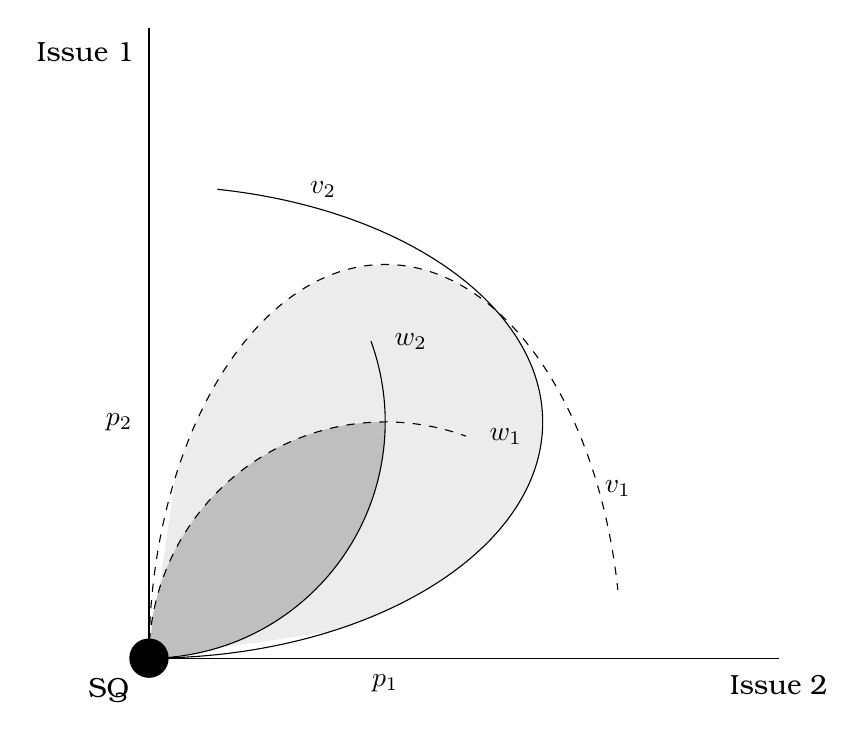
\begin{tikzpicture}
    \draw (0,0) -- (0,8) node [below left = .25em] {Issue 1};
    \draw (0,0) -- (8,0) node [below = .25em] {Issue 2};

    \begin{scope}
      \clip (0,0) arc (180:10:3 and 5);
      \clip (0,0) arc (-90:80:5 and 3);
      \fill [gray!15] (0,0) rectangle (10,10);
    \end{scope}

    \begin{scope}
      \clip (0,0) arc (180:10:3);
      \clip (0,0) arc (-90:80:3);
      \fill [gray!50] (0,0) circle (10);
    \end{scope}

    \draw [dashed] (0,0) arc (180:10:3 and 5) node [above = 3em] {$v_1$};
    \draw [dashed] (0,0) arc (180:70:3) node [right = .5em] {$w_1$};

    \draw (0,0) arc (-90:80:5 and 3) node [right = 3em] {$v_2$};
    \draw (0,0) arc (-90:20:3) node [right = .5em] {$w_2$};

    \node at (0,3) [left = .25em] {$p_2$};
    \node at (3,0) [below = .25em] {$p_1$};
    \fill (0,0) circle (0.25) node [below left = .5em] {SQ};
  \end{tikzpicture}
  \caption{A Two Dimensional Spatial Model}
  \label{fig:twodimensions}
\end{figure}

The winset when both issues are weighted equally by both actors is nested within the winset for when the issues are weighted differently. Thus when actors attach different saliences to different issues they are willing to accept a decrease in utility on one issue for a correspondingly greater gain in utility on a second issue, hence the possibility for striking a deal increases substantially. This is represented by the shaded areas in Figure \ref{fig:twodimensions}, where the darker shade marks the winset when both issues are weighted equally, and the lighter shade marks the winset when one dimension has a higher salience. 

The added value of this model is that it does away with the assumption of sincere voting, which was made in the simple one dimensional spatial model. The results from the two dimensional spatial model are often used when scholars want to explain the prevalence of unanimous decisions in the Council \citep{MattilaLane2001,KonigJunge2009}. However for log rolling to be possible certain conditions need to be fulfilled, first actors need to know each others positions and saliences attached to these positions. Secondly the saliences must differ across actors. If actors are uncertain or do not have access to information on positions and saliences then no log rolling can take place. Third, log rolling in the spatial model is simultaneous. If the votes on the different issues are separated in time then we need to assume that actors can make binding agreements, otherwise one actor will always be able to defect from the deal without incurring any penalties. However the further the votes are from each other in time, the more uncertain any actor will be about the positions and saliences of the others. Thus from a spatial point of view log rolling should take place either simultaneously or within a short time span. 

The spatial model has provided many insights into decision making in legislative bodies, however the model also displays several weaknesses with regards to decision making in the Council.  First of all the simple spatial model is a poor predictor of the level of conflict when the Council votes. The more sophisticated two-dimensional model with varying saliences fares better in this regard, and it does away with the assumption of sincere voting. However the two-dimensional model assumes that log rolling is done practically simultaneously, and thus do not allow for log rolling on situations where there is uncertainty with regards to the issues considered, or when there is a time gap between the consideration of issues. As Keohane has noticed, if only synchronous exchange is possible few agreements would be made, as issues often arise sequentially, hence an appropriate exchange may be impossible when only considering issues at one point in time \citep[21]{Keohane1986}. 

A particular weakness with the spatial models, indeed most formal models, is that they do not provide any clues as to why governments should resort to different types of dissenting votes. The spatial model only predicts whether a government should vote no or yes, however it does not address the issue of abstentions and no votes and how the meaning of these votes change with different voting rules. Spatial models do not necessarily exist in a binary world where governments are either in favor or not. It is conceivable that a criteria could be used to predict when a government would vote no or abstain, based on the distance from the ideal point to the likely outcome. However this challenge has not been taken up in the present research on the Council. When researchers use the spatial model to predict outcomes they make the implicit assumption that abstentions can be lumped together with no votes, this ignores a lot of information  

\section{Diffuse Reciprocity}

\citet{Keohane1986} has labelled the form of log rolling predicted  by the spatial model for specific reciprocity, i.e. an exchange of votes which do not carry any further obligations. He argues that when exchanges do not carry any future obligations only limited cooperation among actors is possible. In this sense synchronous log rolling cannot lead to stable patterns of cooperation. If log rolling is supposed to happen on issues separated in time then a different mechanism is needed. Keohane labels this diffuse reciprocity. The concept of diffuse reciprocity is based around the idea of future gains. It is assumed that actors care about future interactions with each other, and thus they have an incentive to engage in compromises in order to build up a ``favor bank'' which can called upon when the need arises \citep{Heisenberg2005}. Indeed diffuse reciprocity is modelled around a sequential bargaining model where concessions in bargaining exchanges do not have to be made simultaneously nor necessarily be strictly equivalent \citep{Jonsson2000}.  Just like the two dimensional spatial model with differing saliences among actors enlarged the winset, diffuse reciprocity enlarges the number of potential deals to be made by including future bargains into the considerations of actors. 

Within sociology and anthropology the idea of diffuse reciprocity has a long tradition. Starting with the study by \citet{Mauss1950} of the \textsl{potlach} tradition among north american indians and the study of the kula exchange ring among the trobriands of the western pacific by \citet{Malinowski1922}, it has been recognized that asynchronous exchanges contribute significantly to the stability of social systems. In the words of Gouldner:

\begin{quote}
  ``Insofar as we live under the such a rule of reciprocity, when one party benefits another an obligation is generated. The recipient is now \textsl{indebted} to the donor and he remains so until he repays. Once interaction is seen as taking place over time, we may note that the norm of reciprocity so structure social relations that, between  the time of Ego's provision of a gratification and the time of Alter's repayment, falls the shadow of indebtedness.''
\flushright{ - \citealt[174]{Gouldner1960}}
\end{quote}

\citet{Blau1964}, in his theory of social exchange, argue that once a donor-recipient relationship has been established a positive feedback mechanism is set in motion that require actors to further engage in asynchronous exchange relations in order to reap the benefits of the exchanges made. This fosters the development of a social structure in which reciprocity is a defining principle that regulate social interaction. What distinguishes social exchange from purely economic exchange is that economic exchanges are governed by a precise definition of any possible future obligations that might arise as a consequence of an exchange (such a taking a mortgage to buy a house), whereas social exchange involves a general expectation of a future return it is not precisely defined what this return might be. Thus social exchange creates diffuse future obligations, this requires a degree of trust in other actors that they will honor the obligations. It is therefor the inherent risky nature of social exchange relations that make the development of diffuse reciprocity possible \citep[94]{Blau1964}. The social exchange model proposed by Blau has been found to be effective in a number of contexts ranging from small businesses and political parties to experimental settings involving college students \citetext{for an overview see \citealt{CropanzanoMitchell2005}}.  

Many scholars have argued that specific reciprocity can under the right conditions transform into a stable system of diffuse reciprocity \citep{Gouldner1960,Axelrod1986,Keohane1986,NowakSigmund1998,Diekmann2004}. For instance Keohane follows Blau in arguing that when bargaining takes place sequentially there will always be an element of trust between actors. This trust element is found in the build up of a series of debts and credits, where the debtor has an incentive to default. However if there is a high chance of actors to meet again in future negotiations, the shadow of the future will weight heavy on the promises made. If the future is considered sufficiently important then the shadow of the future will outweigh the incentive to defect. This argument is supported by \citet{FehrFischbacherGachter2002} who argue that if the chance of two actors repeatedly interacting with each other is sufficiently high, actors will engage in reciprocal acts of cooperation. \citet{NowakSigmund1998} showed that a reputational mechanism can explain the efficacy of diffuse reciprocity. The crucial aspect of a reputational mechanism is the presence of an audience that witnesses the interactions that a given actor engages in. This allows actors to accumulate ``image'' scores for every cooperative action they make, thus making it more likely that other actors that are aware of their images will cooperate. Such a mechanism only works under the scope conditions that all interactions are done in public and all actors belonging to a group  have the possibility of gaining information on interactions by either observing them directly or by talking to other group members. This argument has also been taken up by Putnam who argues that diffuse reciprocity helps to amplify reputations of actors, and thus makes it easier to overcome dilemmas of collective action \citep{Putnam1995}. As \citet{Axelrod1986} points out, reputations serves as signaling devices, indicating which actors can be trusted in future negotiations an which actors are to be shunned. If an actor decides to default on an obligation this sends a signal to other actors, when a series of donor-recipient relations has been forged this can be very costly for the actor who defaults as s/he might not see any future return on the concessions made.    

Much like log rolling there are thus certain conditions necessary if diffuse reciprocity should develop. First of all actors need to be in an institutional environment in which they will on a regular basis interact with each other. When this condition is fulfilled the shadow of the future will show a strong presence. Furthermore \citet{Lewis2005} argue that actors involved in negotiations need to be in a relatively insulated setting, such that negotiations can take place free of domestic publics bearing witness. 

These scope conditions are to a large degree present in the Council. The permanent representatives meet on a frequent basis in the COREPER I and II committees, and the work of the committees is sheltered from any outside view. It has been shown in the literature on the Council that the frequent meeting activity has led to the rise of a bargaining culture where a vote is seldom pushed, but rather negotiations are carried on until either everybody is on board, or all possibilities has been exhausted \citep{Lewis1998,Lewis2003, BjurulfElgstrom2004}. Moreover the insulation of the COREPER committees allow national representatives  a degree of freedom to pursue deals that might otherwise not be considered by the minister at home, and present them as the best possible outcome \citep[947]{Lewis2005}. This type of consensus seeking bargaining relies heavily on a diffuse reciprocity mechanism. In order to reach a consensual outcome in the light of strong opposition from some governments, it is important that these governments can compromise on their positions and feel secure that they will somehow be compensated at a later date. 


\section{Diffuse Reciprocity and Signaling}

One apparent weakness of diffuse reciprocity, as outlined in this chapter, is the reliance on the recollection of previous negotiations, some often quite a while back in time. Representatives of governments in the Council have limited memories, and they do change from time to time, hence letting it be known that a government is compromising only through verbal agreement can be a risky strategy. Thus an instrument that records the disagreement is a very useful tool. The voting records in the Council is such a tool. Through the registration of a vote governments can leave a permanent record of their behavior. Given the tendency in the Council to have oversized majorities, the voting behavior of the individual government rarely will effect the outcome of a vote, and hence voting records are mainly useful as signaling devices.

Governments in the Council face two audiences, their domestic public and the other governments in the Council. Given that EU politics is seldom placed high on the public agenda, the domestic audience can in many instances be reduced to specialized interest groups. Any government must balance its behavior in the Council between being a credible coalition partner and not offending domestic interest groups. Whenever a government finds itself in the minority position in the Council it must decide whether to silently agree with the majority, somehow show its disagreement while still playing cooperatively, showing open disagreement to the members of the Council, or siding with a domestic constituency against the majority in the Council. Under QMV voting no and abstaining has the same effect, but arguably voting no to a dossier sends a stronger signal to a domestic constituency, which might not be familiar with the procedures in the Council. Other representatives in the Council are likely to grasp the difference, hence when governments want to show strong disagreement within the Council, but not necessarily to the public, abstentions will be the preferred signal. Therefor it makes sense to distinguish between no votes as signals to domestic constituencies and abstentions as signals to other colleagues in the Council. 

Under unanimity the situation is different, however the voting behavior can be interpreted as sending the same signals as under QMV. Any government is a veto player and can block a decision they are not satisfied with, although in praxis this is observed very rarely as most dossiers that cannot be passed in the Council are returned to the Commission to be redrafted. Thus we should only on rare occasions observe no votes under unanimity. Abstentions under unanimity cannot block a decision, thus they are equivalent to a government not being present for a vote and allow the other governments to proceed with the decision. Abstentions, though, do not encourage a decision either hence there is still a substantive difference between abstaining and voting yes. In this sense abstaining is equivalent to sending a signal of dissatisfaction to the Council. 

There is a third option which we have not broached so far. In the Council it is possible to attach statements to votes. Such statements can serve a number of purposes. They are frequently used to illuminate how a given government will interpret certain articles, or how the implementation might differ from other member states. The Council as a body do also frequently attach statements to votes that are typically directed at the Commission. One type of statements that are of particular interest from our point of view is the negative statement. Sometimes governments will attach statements to their votes explaining why they felt compelled to vote the way the did. When a government chose to record a dissenting vote, such statements often describe either fears that a given dossier will create a undesirable precedence within the Community, or that aspects of the dossier are viewed as detrimental to the interests of said government. More often than not governments will attach statements to yes votes detailing aspects that they are not satisfied with. These types of situations speak directly to the argument that governments build up favor banks within the Council, by showing that often governments will agree to vote affirmative to dossiers that they are not satisfied with. 

Finally voting yes in the Council can be interpreted in two ways, either a given government simply do not attach enough salience to a given dossier to raise any objections, or the final outcome is in agrement with the preferences of said government. This is a more complicated case as without information on the salience a given government attached to the dossier we cannot distinguish between the two reasons behind a yes vote. In any case voting affirmative in the Council is less interesting case as it does not provide any meaningful information with regards to signaling behavior. Based on these considerations Table \ref{tab:signaling} show a typology of Council voting behavior based on signal type, recipient and message.

\begin{table}[htp]
  \centering
  \resizebox{\textwidth}{!}{
  \begin{tabular}{l c l} \toprule
    Signal & Recipient & Message \\ \midrule
    No Vote & Domestic Constituency & Support of domestic interests against the Council \\
    Abstention & Council & Strong disagreement with the final outcome \\
    Yes + Negative Statement & Council & Support despite disagreement \\ \bottomrule
  \end{tabular}
}
  \caption{Types of Signaling in the Council}
  \label{tab:signaling}
\end{table}

In Table \ref{tab:signaling} only the third choice category is engaging in an exchange relation within the Council. When a government votes yes to a dossier in which it has reservations and goes through the trouble to make the Council aware of these reservations, it is difficult to explain this type of behavior from a spatial point of view. The simple one-dimensional model cannot accomodate any cases like this. The two-dimensional model is able to accommodate log rolling, however since log rolling is based on an already agreed trade it is difficult to explain why governments would feel the need to advertise their disagreement with the given dossier. The third category is, however, consistent with an explanation of negotiations in the Council based on diffuse reciprocity. Since governments make concession based on diffuse future rewards, it makes sense that they would want to remind their colleagues about the concessions made, and have a permanent record of the concessions. 
 
No votes and abstentions, on the other hand, should both be seen as deviating acts from the diffuse reciprocity mechanism. However deviations comes at a cost. Any deviation from diffuse reciprocity will diminish the number of favors that can be called upon at a later stage, and if done often enough it would put a given government at a severe disadvantage. Only in situations of either severe domestic pressure, or very strong preferences that are not accommodated by the Council, would we expect to see governments compromise their standing within the Council. 


\section{Normative Behavior and Diffuse Reciprocity}

Diffuse reciprocity as defined above is closely associated with the rise of social norms. Indeed Lewis notes:

\begin{quote}
  ``[...] informal norms such as diffuse reciprocity operate in the context of COREPER's institutional environment and can promote pro-norm behavior.''
\flushright{- \citealt[964]{Lewis2005}}
\end{quote}

Most authors view diffuse reciprocity as an expression of a social norm \citep{Keohane1986,Lewis2000,Lewis2005,Diekmann2004}. However, before we can claim that diffuse reciprocity is a social norm we need to carefully define what a social norm is. When discussing norms there is an important distinction between private and social norms. Private norms refer to self-imposed standards governing only an individual, and usually sustained by feelings of guilt and/or anxiety \citep[100]{Elster1989}. Social norms, on the other hand, governs behavior within groups, and are sustained by approval or disapproval by the members of the group towards the actions of the individual. This general definition of social norms is widely shared in the literature \citep{Elster1989,Bicchieri1990,Coleman1990}, however when it comes to the specifics there are many differences. Coleman distinguishes between prescriptive and proscriptive norms, and Elster develops a complex classification scheme for different kinds of social norms. The most specific definition of a social norm is found in \citet{Bicchieri2006} who develops her definition around the idea of expectations and conditional preferences. According to Bicchieri we can define behavioral regularity $R$ in population $P$ as a norm if:

\begin{enumerate}
\item Almost every member of $P$ prefers to conform to norm $R$ on the condition that almost everyone else conforms too.
\item Almost every member of $P$ believes that almost every other member of $P$ conforms to $R$.
\end{enumerate} 

The same conditions that allow diffuse reciprocity to emerge also support the existence of social norms. Indeed diffuse reciprocity is based on the expectation that in the future the exchange will be reciprocated. In order for diffuse reciprocity to work this expectation has to be almost universally shared in a given group. Hence the way diffuse reciprocity is treated in the IR and EU literature aligns it closely with Bicchieris definition of a social norm. 

The advantage of Bicchieris definition of social norms is that it circumvents the problem of internalization. To illustrate this issue consider the popular ``three step model'' of norms \citet{Finnemore1998}. First a norm is promoted through norm entrepreneurs, if they are successful and reach a critical mass, a norm cascade will follow in which more and more actors adopt the norm, in the final step the norm is internalized and becomes habitual. In this model only norms that are successfully internalized will survive and become established modes of practice. Thus in the third step norms become habitualized and are no longer consciously used by actors. The main problem with a model that relies on the internalization of norms is that it makes norms hard to observe, precisely because of their ``taken-for-grantedness'' \citep[495]{Johnston2001}. Furthermore there is plenty of theoretical and empirical evidence that internalization of norms can happen, but is not a necessary condition for norms to thrive. Hence adding an internalization step to a model makes it more complex than need be. It is a long established result in the game theoretical literature that norms can come into existence through the interaction between actors, for instance in the classic tournament by conducted by \cite{Axelrod1986} a cooperation norm can be established simply through actors monitoring each other an adjusting behavior accordingly. Several mechanism are proposed that can sustain norms, among others: reputation and social proof. This is corroborated by Bicchieri who convincingly argue that the rise of a social norm is best viewed as a learning process. When actors engage with each other repeatedly, they build up knowledge of past interactions which can be used to form expectations of future interactions. In this sense social learning has a decidedly bayesian flavor where expectations are continuously updated based on the latest interaction. Hence a norm do not need to be internalized in order to be effective in structuring the behavior of actors.  This is in agreement with the many authors who find that there is a large degree of strategic thought behind normative behavior. \citet{Schimmelfennig2003} find that governments during the debate about eastern enlargement would invoke constituent norms of the EU, such as inclusivity, to further their cause. The same pattern has been observed in the US Supreme court, where the chief justices Marshall and Hughes both used the ideal, that the highest court in the US should present a unified front to the public strategically to ensure unanimous voting decisions \citep{CalderiaZorn1998,Epstein2001}.  


\section{Measuring Diffuse Reciprocity}

In the social sciences social norms have featured prominently in many theories, however when empirically testing social science theories finding an appropriate indicator for normative behavior has not been easy. Two approaches have achieved some prominence. First of all many game theorists have devised different types of games to elucidate normative behavior, typically these games have been used in laboratory settings, where the conditions for normative behavior can be controlled. Based on insights from these experiments one set of authors have devised an approach that involves identifying behavior that is at odds with the preferences of actors. Another set of authors have looked towards the econometric literature on co-integration \citetext{see \citealt{Beck1992}}, and argue that consensus norms regulate conflictual behavior, and if we can identify and underlying factor regulating conflictual behavior, then we have corroborative evidence for the presence of a norm. 

When assessing the causal impact of norms, researchers has often turned to devising experiments under which the conditions for normative behavior can be controlled in an exact manner. In the experimental game theory literature a number of experiments have been devised to elucidate different types of pro-norm behavior ranging from altruism to conditional cooperation. Particularly public goods experiments have yielded interesting insights into how norms are sustained in small groups A common experiment is to let two players play a prisoners dilemma game, where if they cooperate the good is provided and they each share the cost, if one defects the other actor will bear the burden of providing the good. To this setting a neutral observer is added who could decide to punish players at will. Punishment is costly, however, and whenever the observer decided to punish a small cost was incurred. Results from these experiments show that often third parties decide to punish actors that defect, thus lowering the payoff associated with defection \citetext{see \citealt{FehrFischbacher2004} for an overview}. These experiments illustrate that acting normatively often means compromising on pure utilitarian goals, i.e. when the chance of getting caught is high and punishment probable if caught, actors will choose to cooperate. Hence the empirical implication of these experiments is that to observe normative behavior we must identify situations where actors in public settings will act against their own selfish interests.  

This approach, which we can label the direct indicator, has been taken up by \citet{EpsteinSegalSpaeth2001} in their study of the US Supreme court. In the years 1800 to 1942 the US Supreme court had a yearly average of 91.5\% consensual decisions. This is in stark contrast to the period after the second world war, where disagreement has been the rule, not the exception.  Many scholars have argued that there were a norm of consensus present in the Supreme court, however conclusive evidence has been scarce \citep{Haynie1992,EpsteinKnight1996,CalderiaZorn1998,Epstein2001}. \citet{Epstein2001} propose that in order to establish the presence of a norm, one must be able to identify one type of behavior that is only consistent with a normative based explanation. This allows a researcher to dispose with alternative explanations that might produce the same outcome, but through a different mechanism. The approach taken by \citet{Epstein2001} was to identify cases in which judges had expressed doubts about a ruling in private, but still voted with the majority in public.  They argue that:

\begin{quote}
  ``This is precisely the sort of behavior we would expect to find if a norm of consensus operated on the Court; public unanimity masking private disagreements.''
\flushright{- \citealt[365]{Epstein2001}}
\end{quote}

This type of argument is very much in line with the evidence presented in the experimental game theoretic literature on normative behavior, i.e. we can recognize normative behavior when actors engage in costly behavior that is against their own utilitarian preferences. In the Council we have a direct equivalent to the indicator used by Epstein et al. Although the representatives of the governments do not record in detail their discussions, their use of statements attached to their votes indicate whether they acted against their short term interests. On many votes where member states votes yes, we see statements such as the following attached.

\begin{quote}
  ``The Spanish delegation states its disagreement with the distribution of EU TACs in the North Sea and the Baltic Sea areas. Spain maintains the appeals it has made to the Court of Justice of the European Communities against Regulations (EC) Nos 2341/2002 and 2267/2003, under which Spain was granted no quotas in those fishing areas despite the transition period’s having ended, and it will submit a further appeal.''
\flushright{Spain, COM (2004) 785}
\end{quote}

The above quote is taken from the vote on the regulation fixing the fishing quotas for 2005 in waters where catch limitations are required.  During the Spanish and Portugese accession negotiations a transition period was determined where fishing fleets for the two member states where not allowed to fish in the North and Baltic seas. This transition period has already expired, however since Spain commands the largest fishing fleet in the EU other member states have been reluctant in granting the spanish fleet fishing rights i their waters. However despite the efforts of Spain to secure fishing rights in the North and Baltic seas, the spanish government still voted yes to a proposal that did not grant them these rights. The dossier was adopted under QMV, so there was little to be gained from voting no, beyond sending a signal to the Spanish fishermen. Since Spain at the time had a series of appeals running at the European Court of Justice, one could argue that the fishing lobby had been appeased, hence voting yes on this dossier is difficult to explain from a spatial bargaining model, however it  is consistent with an explanation focusing on diffuse reciprocity. 

The second approach, which we can label the indirect indicator, to measuring norms has primarily been used within the IR literature \citep{RajmairaWard1990,RajmairaWard1992, Goldstein1991,Rajmaira1997} and the study of the US Supreme court \citep{CalderiaZorn1998}. The early move within the IR literature to assess the empirical presence of norms was very much influenced by the work of \citet{Keohane1986} and \citet{Axelrod1986}. The authors in the field commonly argue that norms should be viewed as social institutions. As such the purpose of a norm is to structure interaction among participants whenever there is the potential for conflict. Following the classic exchange theorists they argue that social institutions represent equilibrium points, and these equilibrium points are the result of a series of exchanges between actors. Social institutions must be able to engender compliance, otherwise they would not exist for long. In equilibrium compliance can be achieved in two ways. First of all it might be that no actor has any incentive to leave the equilibrium, i.e. to break the norm. The equilibrium point is then the optimal course of action. In this sense norms can be largely self-enforcing. Secondly, norms as institutions can provide reasonable expectations towards the behavior of other actors in certain circumstances. As such a norm will drastically lower the uncertainty that is associated with calculating consequences of possible avenues of action. Finally a norm can come with a sanctioning mechanism. If participants have the possibility to monitor social interactions and detect defection from the rule, sanctioning defectors allows a social institution to be upheld, despite not being the optimal course of action for all participants. In line with the literature on the consensus norm in the Council, all scholars stress the importance of time when dealing with norms. Social settings in which the actors interact frequently, where there is little replacement and socialization takes place by learning from more experienced actors, we can expect a long institutional memory to persist. It is under these conditions that we would expect norms to emerge, and the claim is that we can witness manifestations of norms in the behavior of participants in a social institution over time. The authors argue that a consensus norm should operate by regulating the amount of dissent expressed openly, furthermore this regulation of dissenting behavior should be present in a long time series. To assess this empirically scholars have conceptualized normative behavior as reactive sequences over time. For instance \citep{RajmairaWard1990,RajmairaWard1992} examine Soviet-US relations through the joint-event history of the two superpowers, by coding actions as either reciprocal or conflictual they examine the two time series to see whether they share an underlying component. If the two series tend to drift in the same direction, allowing for short term fluctuations, this evidence of a shared norm of reciprocity. Rajmaira \& Ward find this relationship to be strong in super-power interactions, an show that the past history of interactions are important in forming future expectations. Depending on the history this can lead to either long-term cooperation or conflict, as expectations become self-fulfilling. A similar pattern has been found in the US Supreme court by \citet{CalderiaZorn1998}. In the Supreme court judges have three possible choices when casting their vote, they can vote yes, no or write a concurrent opinion in which a judge expresses his/her agreement with the majority, but with different reasons as the basis for the decisions. Calderia \& Zorn argue that if a consensus norm is present in the Supreme court, then it should express itself in a consistent low level concurrences and dissenting votes, and both series should be governed by the same underlying factor. They find a strong relationship between concurrences and dissenting votes. This is interpreted as evidence for the presence of a consensus norm. This approach to measuring norms as the underlying factor the binds together long term trends in behavior that is consistent with normative expectations, carry a high potential for research on the consensus norm in the Council. Very much like the US supreme court, the copiously large amount of consenting votes have been interpreted as evidence for a consensus norm. In order to determine whether it really is a consensus norm that governs the high number of yes votes, the literature on norms in IR and the US Supreme court show that we can gain much by focusing on the relationship between types of dissenting votes. 

What type of norm the approaches outlined above capture is not clear. One assumption made in all studies is that we can identify one area of interest which should be governed by a single norm. Both Epstein et al. and Calderia \& Zorn assume that there is only one norm operating within the Supreme court, namely a consensus norm. In the same vein Rajmaira \& Ward assume that their tests capture a norm of reciprocity. In this chapter I have argued that a norm of diffuse reciprocity is the most likely explanation for the consensus seeking behavior in the Council,  this implies that any evidence found of normative behavior in the subsequent chapters will be interpreted as corroboration that a norm of diffuse reciprocity is active in the Council. 

\section{What to Come}
This chapter laid out the micro foundations for a theory of diffuse reciprocity within the Council. By showing how diffuse reciprocity can come into existence through exchange relations, and once established can lead to asynchronous log rolling, the foundations for an explanation of consensual voting in the Council relying on informal norms and methodological individualism was specified. Under a regime of diffuse reciprocity where any single vote will rarely make a difference, and governments use different types of dissenting that are formally equivalent, treating votes as signaling devices provides a possible explanation of the voting patterns that has been observed in the Council.  

In the next chapters the theory developed here will be explored with regards to three different aspects of decision making in the Council. Chapter \ref{chapter:votechoice} will examine the determinants of vote choice in the Council. A key aspect of the diffuse reciprocity approach to negotiations in the Council is the vote choice of the member states governments, if these choices are indeed signaling devices then we should be able to explain the vote choices as functions of domestic concerns, governments preferences and council composition variables.

In chapter ?? we will utilise the direct indicator, to determine the effect of diffuse reciprocity on the decision making speed of the Council. Several pieces have suggested that diffuse reciprocity has an effect on decision making time, if these claims are correct we should be able to explain decision making time as a function of diffuse reciprocity.

Chapter ?? will examine the time dependent aspect of diffuse reciprocity through the indirect indicator uncovered above. DIffuse reciprocity is build around the idea of asynchronous exchanges, hence time is a crucial aspect of the theory. Over time we should expect that the norm of diffuse reciprocity is effective in keeping dissenting votes at consistently low levels in the Council. Following the indirect indicator approach this translates into treating abstentions and no votes as two time series that share a common regulating factor. 

For each chapter the theory is extended and testable hypotheses are developed based on the premised laid out in this chapter. 



\chapter{Determinants of Vote Choice}
\label{chapter:votechoice}

\lettrine{T}{he} Food Flavoring directive adopted in 2008 was a controversial dossier. Especially Germany had issues surrounding the levels of allowed additives derived from aromatic spices and herbs. The dossier was adopted unanimously in the Council, but the German government attached the following statement to their vote. 

\begin{quote}
  ``Germany would have preferred a lower coumarin limit for traditional and seasonal bakery ware containing cinnamon the the one now provided for, but in a spirit of compromise can nevertheless support the proposed maximum level''
\flushright{ - Council Monthly Summaries October 2008 p. 21}
\end{quote}

 The dossier had been debated in the Council and parliament since 2006 and the parliament had significantly strengthened the scope of text from the Commission. Among other things, the Parliament proposed to leave an annex regarding the risk of using certain aromatic herbs and spices open until further evidence could be provided to determine the appropriate risk levels. This was welcomed by Germany which had argued that the levels set in the Commission proposal with regards to cinnamon were too high. However the Parliaments amendments was met with opposition from other governments in the Council, who feared that traditional artisans that produced bakery goods with cinnamon would be unnecessarily burdened by a lower limit.  Recognizing that the Council could not reach a decision the Commission withdrew the proposal, to redraft it. After several debates in the Council Germany agreed to give in on its reservations. 

The voting behavior of Germany on the Food Flavoring directive represents a case where  ....

This sort of behavior is an aspect of decision making not captured in current studies of the Council.  Most studies so far only examine yes votes, no votes or abstentions, thus situations like the one above where Germany expressed strong reservations about the legislation, but still voted yes, are not captured. Including cases like the one above thus allows us to study voting behavior in a more fine grained manner.

It is a commonly used explanation whenever a pattern of consensus is found in the Council to refer to the consensus norm, and often the high degree of unanimously adopted dossiers in the Council is used as corroborating evidence. However using unanimously adopted decisions as evidence for a consensus norm is not without pitfalls. There are many reasons for why a dossier was adopted unanimously. A dossier could be uncontroversial, thus requiring no need for seeking consensus. It is also possible that the preferences where so aligned that an agreement was reached without needing to resort to long negotiations. Finally it might be that logrolling was the mechanism. 

The cases of inflating a data set with uncontroversial dossiers or dossiers where the preferences were aligned can be remedied at the case selection stage. To distinguish between logrolling and diffuse reciprocity it is argued that behavior of the type exhibited by Germany above can be interpreted as engaging in diffuse reciprocity, by building up the ``favor bank''. 


\section{Diffuse Reciprocity and Voting in the Council}

Social norms offer consideral scope for interpretation, manipulation and choice. To treat norms as monolithic entities that determine social interactions is to revert back to the fallacy of the over-socialized actor that has plagued much of constructivist theory, however to treat norms purely n as tools to mask self-interest is to make the fallacy of the under-socialized actor plaguing much of rational choice theory \citetext{see \citealt{Elster1989} and \citealt{Schimmelfennig2000} for good overviews and critiques}. The theory of diffuse reciprocity is based around the notion of unanticipated consequences, as exchanges aquire a decidedly social flavor, actors get caught up in the emerging system of debts and credits. It is important to keep in mind that at no point are actors aiming towards such a system, it is an emergent phenomena resultant from the interactions in a social system. Since diffuse reciprocity do not rely on the internalization of a social norm, it is closer to a social equilibrium in which most actors would be worse of if they engaged in off equilibrium behavior. In such a system it is always a possibility that a government choose to pursue its own interest in hope of some short term gain, if the expected gain is higher than the expected long term loss in standing. The pertinent question raised here is when will a government decide to deviate from the exchange system, and pursue its own narrow interests. Drawing upon the work in chapter \ref{chapter:theory} we can label the incentives to defect in two categories, namely domestic concerns and preferences. These two categories are not entirely mutually exclusive, it is possible that domestic concerns will align with strong preferences against the final outcome. Furthermore the two categories are roughly correspondent to the classic concerns over whether politicians are mainly driven by the wish to succeed electorally, or to influence policies \citep{Strom1990}. There is evidence for both types of motivations in the literature on coalition formation, for instance \citet{MartinStevenson2001} show that parties, when deciding with whom to create a coalition, will show concerns for which office they will hold and the policy content of the coalition. In the Council concerns about electoral success can manifest themselves when domestic politics and EU legislation collide. This can often put governments in delicate situations where they must choose between being good members of the EU and appeasing domestic constituencies. The trouble of the reintroduction of the border control at the Danish border is illustrative in this regard. As part of a domestic settlement the Danish government agreed to introduce a limited border control in order to get the votes from the nationalistic Danish Peoples Party (DPP). Since Denmark is a member of the Schengen area, the implementation could only be very limited if should be complient with Schengen rules. However at home the DPP was claiming that the border controls would be a return to the border control that was in place befor Denmark joined the Schengen area \citep{Olsen2011,Euractiv2011}. This put the government in a difficult position where it had to choose between either downplaying the role of the border control, which would offend the DPP, or going along with the DPPs claim which would offend the Commission. 

Governments in the Council face two types of domestic constraints. One type can be labelled interest group pressure, and is distunguished by strong interest groups pushing an agenda at the EU level that is not necessarily in line with the preferences of the government. Lobbying has long been part of negotiations in Brussels. Lobbying typically display a pattern where national interests, organized in an umbrella organization, will go through their European counterpart to influence policy makers in Brussels. However often national umbrella organizations will also contact the relevant national ministers directly in order to convince them to push an agenda in the Council \citep{Beyers2002}. Most often interest groups will focus their attention on changing parts of the legislative text that they are not happy about, however when these efforts have proven futile the focus might be on recommending a government to vote no as a signal of support for domestic concerns. This has the effect of building relations between key constituent groups domestically, but will lower the standing of the government in the Council. The other constraint can be labelled public opinion. If a dossier at the EU level catches the eye of the public in a member state, it can have an impact in the re-election concerns of governments, particularly on EU sceptic member states such as the UK and Denmark. An interesting dynamic that has often been observed in the Council is blame shifting. In multilevel systems it is easy for institutions at at given level to engage in blame shifting and credit taking for political outcomes \citep{Anderson2006}. This has been observed in member states where governance is divided between different administrative structures, such as France and Germany \citep{Elgie2006}. It is no surprise that the same dynamic has also been oberserved to take place between member states governments and the EU \citep{Franchino2004}. If governments find themselves under pressure domestically, but are unable to block legislation at the EU level, it is tempting to vote no in order to appease the domestic audience, and blame the EU for forcing unwanted legislation. 

In the absence of domestic constraints, governments migh find themselves highly disagreeing with the outcome. The theory of diffuse reciprocity will predict that in these situation, the vote choice is dependent upon how much the future is weighted. If an actor has been very active in maintaining exchange relations then the future is weighted heavily, thus we would expect this actor to compromise. However actors that are not active in the system of exchanges will not weight the future very heavily, hence we will expect these actors to vote more along their preferences. This line of argument has been developed by \citet{HoylandHansen2010}. They argue that the consensus norm in the Council can be viewed as the propensity to override once own preferences in favor of a consensual decision. They are thus in line with the direct indicator approach specified in chapter \ref{chapter:theory}. In order to further specify this mechanism the authors use a spatial model with an added term to capture any effect of a consensus norm. Assuming that actors operate in a one-dimensional space with a linear loss function, the principle of utility maximization implies that an actor $i$ will vote yes to a dossier if:

\begin{equation}
  \label{eq:1}
  U_{ik}(-|x_{ik} - p_k|) < U_{ik}(-|x_{ik} - q_k|)
\end{equation}

Where $U_{ik}$ is the utility of actor $i$ on dossier $k$, $x_{ik}$ is the ideal position of actor $i$ on dossier $k$, $p_k$ is the position of the proposed dossier and $q_k$ is the status quo. Equation \ref{eq:1} thus represents the classic spatial model, to account for the effect of the consensus Hoyland \& Hansen add a third term, $\theta$, which is added in linear fashion to the loss function. Hence:

\begin{align}
  \label{eq:2}
  U_{ik}(-|x_{ik} - p_k|) > U_{ik}(-|x_{ik} - q_k|) &= No \\
  U_{ik}(-|x_{ik} - p_k| + \theta_i) < U_{ik}(-|x_{ik} - q_k|) &= Yes
\end{align}

Theta, if positive, will have the effect of reversing the vote, whereas if set to zero or a negative value will have no effect. According to \citet{HoylandHansen2010} if theta is constant across actors this will be evidence of a norm, however the theory of diffuse reciprocity will expect that there is variation in theta, as it more accurately reflects the degree to which a given actor is embedded in an exchange system. The authors do indeed find that theta varies significantly across member states in the Council, this is interpreted as evidence against a consensus norm, although it fits with the theory of diffuse reciprocity. The modified spatial model presented by Hoyland \& Hansen helps to illuminate some of the dynamics that could explain the effect of the consensus norm. However, like the spatial models covered in chapter \ref{chapter:theory}, the approach can only explain the choice between voting yes or dissent. The model do not provide any clue as to why some governments will abstain or vote no on dossiers. What we can learn from the model is that in the presence of a positive theta, only a strong disagreement with the final outcome will result in a government choosing a dissenting vote. 

Based in the above considerations we can formulate the following hypotheses:

\begin{quote}
  H1: When there is domestic pressure governments will vote no on a given dossier
\end{quote}

\begin{quote}
  H2: When governments are preference outliers they will abstain on a given dossier
\end{quote}

The social environment is an important aspect of diffuse reciprocity. Only when actors meet and interact on a regular basis can we expect to see a norm of diffuse reciprocity develop. This is often referred to as a process of social learning. In its most simple form this process assumes what \citet{Skyrms1997} has called Markov agents, i.e. actors that only use the immediate past to adapt their behavior. Social learning in this context is defined by actors interacting and then updating their beliefs about other actors which might lead to a change in their behavior. If this process is run for a long enough period of time, then the interactions will settle on a specific pattern, and we say that the social system has converged. If we assume that actors memory stretches further back than just the immediate past we get actors that condition their future expectations on the past behaviors of their colleagues, which in small groups with a stable membership can lead to the emergence of diffuse reciprocity. The starting point of this causal chain is the interaction frequency, which is a key variable to account for. This opens up the possibility that a norm of diffuse reciprocity might be present to different degrees in different policy areas based on the meeting frequency of the Council configurations. In policy areas where the Council configuration only meet in-frequently we would expect the norm of diffuse reciprocity to be less strong than in policy areas where the Council configuration meet frequently. For instance in 2010 the General Affairs Council meet 16 times while the Economic and Financial Affairs Council (ECON) meet 29 times, hence we would expect that the norm of diffuse reciprocity is more present in the ECON configuration. In voting behavior this would manifest itself in fewer instances of governments voting yes to dossiers, but attaching dissenting statements to their votes. This leads to the following hypothesis:

\begin{quote}
  H3: The higher the meeting frequency the more often we will see governments attaching dissenting statements to yes votes
\end{quote}

%a social dilemma: vote along with preferences for an immediate benefit, or vote against for a diffuse long term benefit. 

%The role of the social environment

%what determines vote choice


\section{Research Design}

\subsection{Case Selection}

In order to test hypotheses about voting behavior in the Council it is important to have the proper universe of cases. In most studies of voting in the Council the focus has been on either the entire population of cases, typically aggregated in some fashion. This ignores the possibility that there might be a great number of dossiers in the Council that are mainly technical, and thus do not engender any deal of controversy from the member states government. In these non-controversial cases we should expect the Council to exhibit perfect cohesion with regards to voting. From our perspective these cases are also not interesting as only in cases with some degree of controversy do we expect the norm of diffuse reciprocity to be active. Hence it is important to be able to distinguish between cases in which the preferences of member states are all aligned, from cases in which there was some degree of disagreement within the Council. Indeed including these cases in the analysis risks biasing the analysis towards finding evidence for a high degree of consensus, and hence stack the deck in favor of a consensus reading of the Council. 

The first step in the analysis is to define the population of relevant cases. In our case the population is defined as dossiers treated in the Council where there was disagreement about the final outcome. In the literature on decision making in the EU several criteria has been used to separate controversial from uncontroversial dossiers. It has been common in the voting record literature to analyze cases on which there was a dissenting vote separately \citep{Heisenberg2005,Hayes-renshaw2006,Hagemann2008}. However this introduces selection bias if the dependent variable is the vote choice of the member states. The DEU project \citep{Thomson2006a} used the criteria of public reporting. If an act was mentioned in Agence Europe it was considered as being controversial. This approach has the drawback that it is not possible to discern whether this controversy represented divisions within the Council, or disagreements between constituent groups and the decision reached by the Council. In order to avoid this ambiguity I will use a more direct measure of controversy within the Council. The cases used in this paper are selected on the basis of having, at one point, been treated as a B point in the Council. The Council agenda distinguishes between A and B points, where A points are dossiers that do not require discussion at the ministerial level, and B points are dossiers in which no agreement could be reached on working group level and need discussion at ministerial level. It is common practice in the Council that issues that are discussed as B points are afterwards send back to the COREPER for a final drafting and than at a later date adopted as an A point in the Council. In recent years several scholars have noted the rise of ``false B-points'' \citep{Muehlbock2011} 

The advantage of selecting only cases treated as B points in the Council is that we are sure to select cases in which there were some controversy related to differences within the Council, and the selection rule does not restrict the variance on the voting outcome. 

There are, however, also issues with the selection rule chosen in this chapter. 

\subsection{Data and Variables}
The dataset used in this paper cover the years 1999 to 2009 and includes every vote in the Council during this time period. In total there are votes registered on 3937 dossiers, which gives a total of 78968 votes cast by member states governments. Of these 16473 where cast for dossiers that at one point was a B point in the Council. Beside the vote cast, the data also contains information on whether a statement was registered by any member state, and whether this statement expressed dissatisfaction with the outcome. This coding is more fine grained compared to most studies who either ignore the possibility of registering a statement in conjunction with a vote, or simply code whether there was a formal statement or not.

The focus of this study is the voting behavior of the member states in the Council of the EU. As such the dependent variable is the individual vote choice of the government in power in a given member state. There are three vote choices available to any member state, namely yes, no or abstain. These choices are coupled with the possibility of also registering a statement in conjunction with the vote. Thus there are six possible combinations of vote and statement:

\begin{enumerate}
\item Yes
\item No
\item Abstain
\item Yes + Statement
\item No + Statement
\item Abstain + Statement
\end{enumerate}

Here we have only included the statements that express dissatisfaction with the final outcome. Thus the dependent variable reflect one category of agreement (yes) and five categories of different types of dissent. It is difficult to rank vote choices, they represent different choices which do not have a well defined high and low point according to which they can be ranked. For this reason the variable is treated as being nominal in this paper. 

The independent variables are measured on two levels, namely the dossier level and the member state government level. The member state government is the lowest level in the data, and are nested with the dossier level, such that for each dossier we have recorded between 15 and 27 votes that are attributed to governments from the member states. A potential biasing factor is the presence of country specific interests in given policy areas. Without very detailed knowledge of the economies of each member state it is difficult to device a measure of national interests across policy areas. Given that the simplest way to control for national interests is to include dummies coding for whether a member state has a large interest in a policy area,  an equivalent approach is to include both country and policy area dummies in the model. However due to  some member state governments not utilizing all voting choices during their stay in office, including country dummies leads to many empty cells, and hence the model cannot converge. Hence the best we can do in order to see if there are any biasing effects is to first conduct an analysis on the full data, without country dummies. Then conduct a separate analysis on a subset of the data only including member states that utilized all voting choices. This is not an ideal solution, but since national interest are only needed as a control it is acceptable in this context. This analysis was conducted and the effects did not change substantially, thus in the analysis below only the Council configuration dummies along with the dummy for dossiers dealing with agriculture and regional policies are included in the models. 

\subparagraph{Left-right} The position of each government was recorded on a 0 tp 10 scale where 0 is the most left leaning a government can be, and 10 is most right leaning a government can be. The data was taken from the ParlGov database (Doring Mannow 2010). Since the variable is recorded on the government level, the same information is also used to calculate the median position with in the Council at any given vote. From this the distance between any government and the Council median was calculated

\subparagraph{Power} To distinguish powerful governments from the less powerful, the raw vote count of a given member state is used. The vote count is based on the population size of a member state, and correlates highly with GDP. The vote is not transformed into a power index as these tend to produce the same ranking as the raw vote count for the Council [REFERENCES] and in order to make the variable more interpretable the raw vote count is used. 

\subparagraph{Presidency} A simple categorical variable coding for which government is holding the presidency is included.

\subparagraph{Net Beneficiary} This variable takes the net amount a member state received from the EU in a given year and subtracts it from the amount paid to the EU. A positive value indicates a net beneficiary, whereas a negative value indicates a net contributor. 

\subparagraph{Agriculture/Regional Policies} A dummy variable distinguishing whether a dossier fell under agriculture or regional policy areas.

\subparagraph{Meeting Frequency} The potential for socialization within a given Council configuration is measured through the number of Council sessions held in a given year. One alternative would be to count the number of Council sessions between the Commission submission of the dossier to the Council and the final vote. However since the socialization argument is cast at the Council level, and not the single dossier, it is more appropriate to use the yearly count of meetings as a proxy for interaction density. 

\subparagraph{Voting Rule} A categorical variable controlling for whether unanimity or QMV was in force in the final vote on a given dossier.

\subparagraph{Type of Legal Act} A categorical variable controlling for whether the Council was voting on a directive, regulation, or decision. 

\subparagraph{Salience} A count variable controlling for the number of times a dossier was discussed at ministerial level. This is not a country specific salience measure, but a measure of how salient the dossier was for the Council as a whole. 

\subsection{Method}

As the dependent variable takes the shape of a nominal variable a multinomial logit is chosen. The multinomial logit model is specifically designed for modeling variables that take the shape of different, non-ranked, choices, also referred to as revealed preferences. The advantage og using a multinomial model over an ordinal is that we do need to assume any type of ranking in the dependent variable, and hence when there is doubt about how to rank a variable this approach is more suitable. Multinomial models are complex beasts, and require care when estimating and interpreting. Since the  model is essentially a series of logit models estimated simultaneously, one for every pair of choices, we have many equations to keep track of \citep[CHapter 6]{Long1997}. It is usual to choose one baseline category, and then estimate all models with this baseline as the reference. Here I have chosen to use the yes category as the baseline, and estimated the 5 equations pairing every other category with the baseline. Thus when interpreting the coefficients in the models, they represent the effects of choosing, say to abstain, compared to choosing to vote yes. 



\section{Descriptive Evidence}
As a first look at the data table \ref{tab:depvar} show the distribution of votes across Council Configurations. The number of yes votes dominates the distribution. Even after having selected only definitive legal acts that where treated as B points in the Council, the number of yes votes is staggering. Surprisingly the second largest category is yes votes that have a dissenting statement attached. This category is in all Council configurations the second largest, and show that studies not taking Council statements into account risk biasing their findings towards consent. The prevalence of attaching negative statements to supporting votes suggests that there is a large degree of signaling behavior going on in the Council. It is important to let your colleagues know that you are a team player and willing to compromise. This speaks fot the interpretation of negotiations in the Council as oriented towards diffuse reciprocity and problem-solving. It is also striking that dissenting behavior is not equally distributed across Council configurations. Agriculture\& Fisheries, Competition and Employment, Health \& Consumer Affairs exhibit a very high degree of dissent when compared to the other Council configurations. Thus we clearly see some policy specific effects on voting.


\begin{table*}[ht]
\begin{center}
\resizebox{\textwidth}{!}{
\begin{tabular}{rrrrrrrr}
  \hline
 & 1 & 2 & 3 & 4 & 5 & 6 & Total\\ 
  \hline
Agri/Pech & 2760 &  92 &  41 &  35 &  17 & 160 & 3105\\ 
  Comp. & 2993 &  20 &  16 &  16 &   7 &  42 & 3094\\ 
  Ecofin & 247 &   0 &   0 &   0 &   0 &   0 & 247\\ 
  Education/Culture & 246 &   2 &   0 &   0 &   2 &   9 & 259\\ 
  Employment/Consumer & 1896 &  26 &  20 &  23 &  18 &  55 & 2038\\ 
  Environment & 1216 &  16 &   6 &  15 &   8 &  20 & 1281\\ 
  Gen. Affairs & 227 &   5 &   0 &   0 &   0 &   9 & 241\\ 
  JHA & 1192 &   2 &   1 &   1 &   2 &  21 & 1219\\ 
  Trans./Energy & 1975 &  12 &  11 &   8 &   3 &  34 & 2043\\ \hline
Total & 12752 & 175 & 95 & 98 & 57 & 350 & 13527\\
   \hline
\end{tabular}
}
\end{center}
\caption{The Distribution of Votes Across Council Configurations}
\label{tab:depvar}
\end{table*}

Table \ref{tab:dissent} lists the ten most dissenting governments in the period 1999 - 2009. The governments were ranked according to how many dissenting votes they had in the Council divided by the number of days they spend in government. The left-right position of the government, the average Council left-right score during the governments stay in office and the deviance between the two scores is also reported. A common finding in the literature on the Council is that large member states are more prone to vote no or abstain than small member states. However if we disaggregate the data into member state governments and adjust for time spend in power, then a different picture emerges. Austria is one of the member states that is usually regarded as being not prone to dissent, but during the short lived second Schuessel cabinet, the government had a series of conflicts in the Council. Moreover the table gives a first hint that there might be an effect of the left-right position of a government on voting behavior in the Council. Except for Schuessel, Verhofstadt and Balkanende, all governments deviate more than one point from the mean Council position, in the case of Schroeder, Persson and Marcinkiewicz more than two points. There are also some hints that member state size, left-right deviation and dissent are related. 

\begin{table*}[ht]
\begin{center}
\resizebox{\textwidth}{!}{
\begin{tabular}{ll c c c p{3cm} p{3cm} p{3cm}}
  \hline
 Country & Cabinet & Ratio & Dissent & Days in Power & Left-Right & Mean Council Left-Right & Deviance \\ 
  \hline
ITA &D'Alema\_I & 0.06 &  25 & 426 & 2.63 & 4.53 & 1.90 \\ 
 AUS & Schuessel\_II & 0.04 &   4 & 96 & 5.20 & 5.75 & 0.55 \\ 
DEN & Rasmussen\_F I & 0.02 &  28 & 1179 & 7.22 & 5.71 & 1.51 \\ 
POL & Marcinkiewicz\_I & 0.02 &   4 & 186 & 7.75 & 5.39 & 2.37 \\ 
BEL & Verhofstadt\_III & 0.02 &   4 & 194 & 5.69 & 5.42 & 0.27 \\ 
SWE & Persson\_III & 0.02 &  28 & 1446 & 3.37 & 5.64 & 2.28 \\ 
GER & Schroeder\_II & 0.02 &  21 & 1127 & 3.24 & 5.69 & 2.46 \\ 
UK & Blair\_II & 0.02 &  26 & 1428 & 4.18 & 5.65 & 1.47 \\ 
NET & Balkenende\_III & 0.02 &   4 & 230 & 5.26 & 5.47 & 0.21 \\ 
FRA & Raffarin\_III & 0.02 &   7 & 427 & 6.80 & 5.61 & 1.20 \\ 
   \hline
\end{tabular}
}
\end{center}
\caption{The Ten Most Dissenting Governments Between 1999 and 2009}
\label{tab:dissent}
\end{table*}

In order to see if the presidency effect is present in the data, the data was split into two groups, one group consisted of all votes in which the government that voted held the presidency, and the other group consisted of all votes in which the government did not hold the presidency. In each group the number of dissenting votes relative to the total number of votes was calculated, and surprisingly there were only minuscule differences between the ratios (0.057 for the presidency group and 0.058 for the non-presidency group). Thus on the aggregate level the presidency does not seem to reduce the level of dissent. However if we examine individual governments there are some differences. When only looking at no votes and abstentions (with and without statements), the Blair II government see a reduction from 0.03 to 0 when holding the presidency. However if we include yes votes with a dissenting statement as part of the dissent category the presidency increases the level of dissent from 0.09 to 0.14. Indeed only examining the yes votes with a dissenting statement, there is an increase from 0.06 to 0.14. Thus there are large effects for some governments, however for most governments this is not the case.


\section{Inferential Analysis}

In order to further test whether the relationships found here hold when controlling for potentially confounding effects, and to test the other hypotheses, a multinomial choice model is used. Table \ref{tab:summary} presents summary statistics for the continuous and count variables used in the model, the categorical variables are excluded. The Hausman test for irrelevant alternatives rejected the null hypothesis, thus the IIA assumption is not violated. Tables a - d in panel 4 show the results from the models. All models include Council configuration dummies, to save space these are not reported. Table a only contain the variables of theoretical interest, tables b - d introduce controls for dossier type, voting rule and salience, table 5 show the full model with all controls Finally table 6 show the full model with all controls, including an interaction term between the power and outlier variables. When including an interaction term in a statistical model the constituent parts of the term can no longer be meaningfully interpreted in their own right. Therefore, in order to be able to evaluate hypotheses one and two, the interpretation will focus on the full model with and without the interaction term.

\begin{table*}[hrp]
\subfloat[Model with Council Dummies]{
\resizebox{\textwidth}{!}{
\begin{tabular}{rrrrrrrr}
  \hline
 & Constant & Outlier & Power & Net Beneficiary & Meeting Frequency & Presidency & Agriculture/Regional \\ 
  \hline
1$|$2 & 2.29 & -0.22 & 0.01 & 0.00 & 0.06 & 0.07 & -0.06 \\ 
          & 5.57 & -2.94 & 1.52 & 1.99 & 1.83 & 0.27 & -0.36 \\
1$|$3 & -0.99 & 0.02 & 0.03 & -0.00 & -0.02 & 0.24 & 0.82 \\ 
        & -1.37 & 0.19 & 1.83 & -0.14 & -0.27 & 0.59 & 3.31 \\
  1$|$4 & -0.78 & -0.06 & 0.03 & 0.00 & -0.07 & 0.18 & -0.12 \\ 
            & -0.88 & -0.34 & 2.08 & 0.48 & -0.90 & 0.34 & -0.34 \\ 
  1$|$5 & -1.07 & 0.03 & -0.03 & 0.00 & -0.04 & -0.20 & 0.47 \\ 
             & -1.24 & 0.18 & -1.42 & 1.28 & -0.52 & -0.36 & 1.50 \\ 
  1$|$6 & -0.12 & -0.05 & -0.01 & 0.00 & -0.17 & -0.31 & -0.11 \\ 
             & -0.10 & -0.27 & -0.55 & 0.11 & -1.68 & -0.41 & -0.24 \\ 
   \hline
\end{tabular}
}
}

\vspace{1em}

\subfloat[Model with Council Dummies and Controlling for Dossier Type]{
\resizebox{\textwidth}{!}{
\begin{tabular}{rrrrrrrrrr}
  \hline
 & Constant & Outlier & Power & Net Beneficiary & Meeting Frequency & Presidency & Agriculture/Regional & Directive & Regulation \\ 
  \hline
1$|$2 & 3.01 & -0.22 & 0.01 & 0.00 & 0.05 & 0.07 & 0.00 & -0.43 & -0.57 \\ 
& 6.18 & -2.97 & 1.56 & 1.98 & 1.31 & 0.26 & 0.00 & -2.08 & -2.93 \\ 
  1$|$3 & -0.10 & 0.02 & 0.03 & -0.00 & -0.03 & 0.24 & 0.89 & -0.82 & -0.78 \\ 
& -0.13 & 0.18 & 1.86 & -0.16 & -0.49 & 0.59 & 3.53 & -2.39 & -2.44 \\ 
  1$|$4 & -0.39 & -0.07 & 0.04 & 0.00 & -0.11 & 0.17 & -0.03 & 1.23 & 0.05 \\ 
 & -0.36 & -0.41 & 2.11 & 0.51 & -1.45 & 0.33 & -0.08 & 2.36 & 0.09 \\ 
  1$|$5 & -0.41 & 0.03 & -0.03 & 0.00 & -0.05 & -0.20 & 0.52 & -0.56 & -0.56 \\ 
& -0.41 & 0.17 & -1.41 & 1.27 & -0.66 & -0.36 & 1.62 & -1.45 & -1.45 \\ 
  1$|$6 & -0.91 & -0.05 & -0.01 & 0.00 & -0.14 & -0.31 & -0.18 & 0.21 & 0.49 \\ 
 & -0.65 & -0.25 & -0.55 & 0.11 & -1.33 & -0.40 & -0.41 & 0.38 & 0.90 \\ 
   \hline
\end{tabular}
}
}

\hspace{1em}

\subfloat[Model with Council Dummies and Controlling for Voting Rule]{
\resizebox{\textwidth}{!}{ 
\begin{tabular}{rrrrrrrrrr}
  \hline
  & Constant & Outlier & Power & Net Beneficiary & Meeting Frequency & Presidency & Agriculture/Regional & QMV & Unanimity \\ 
 \hline
 1$|$2 & 2.74 & -0.22 & 0.01 & 0.00 & 0.06 & 0.07 & -0.07 & -0.46 & -0.63 \\ 
& 4.83 & -2.93 & 1.50 & 2.00 & 1.88 & 0.27 & -0.45 & -1.18 & -1.53 \\ 
  1$|$3 & -1.64 & 0.03 & 0.03 & -0.00 & -0.01 & 0.24 & 0.74 & 0.57 & -1.00 \\ 
& -1.50 & 0.23 & 1.78 & -0.14 & -0.09 & 0.60 & 2.99 & 0.70 & -1.06 \\ 
  1$|$4 & -1.62 & -0.05 & 0.03 & 0.00 & -0.06 & 0.19 & -0.20 & 0.83 & -1.34 \\ 
& -1.15 & -0.31 & 2.03 & 0.48 & -0.84 & 0.36 & -0.58 & 0.76 & -1.03 \\ 
  1$|$5 & -0.35 & 0.03 & -0.03 & 0.00 & -0.03 & -0.20 & 0.34 & -0.73 & -3.54 \\ 
& -0.33 & 0.19 & -1.45 & 1.29 & -0.43 & -0.34 & 1.10 & -1.19 & -3.01 \\
  1$|$6 & -11.48 & -0.05 & -0.02 & 0.00 & -0.16 & -0.31 & -0.14 & 11.33 & 10.69 \\ 
& -0.08 & -0.24 & -0.58 & 0.11 & -1.64 & -0.40 & -0.32 & 0.08 & 0.07 \\ 
  \hline
\end{tabular}
}
}

\hspace{1em}

\subfloat[Model with Council Dummies and Controlling for Salience]{
\resizebox{\textwidth}{!}{ 
\begin{tabular}{rrrrrrrrr}
  \hline
 & Constant & Outlier & Power & Net Beneficiary & Meeting Frequency & Presidency & Agriculture/Regional & B Points \\ 
  \hline
1$|$2 & 2.44 & -0.22 & 0.01 & 0.00 & 0.06 & 0.07 & -0.06 & -0.06 \\ 
 & 5.74 & -2.95 & 1.55 & 2.00 & 1.72 & 0.26 & -0.39 & -1.45 \\ 
  1$|$3 & -1.44 & 0.03 & 0.03 & -0.00 & -0.00 & 0.25 & 0.82 & 0.13 \\ 
& -1.94 & 0.21 & 1.75 & -0.17 & -0.00 & 0.63 & 3.35 & 2.20 \\ 
  1$|$4 & -1.02 & -0.05 & 0.03 & 0.00 & -0.06 & 0.18 & -0.12 & 0.08 \\ 
& -1.11 & -0.33 & 2.06 & 0.46 & -0.82 & 0.35 & -0.34 & 1.11 \\
  1$|$5 & -1.28 & 0.03 & -0.03 & 0.00 & -0.03 & -0.20 & 0.47 & 0.07 \\ 
& -1.43 & 0.20 & -1.45 & 1.28 & -0.42 & -0.36 & 1.51 & 0.85 \\ 
  1$|$6 & -0.12 & -0.05 & -0.01 & 0.00 & -0.16 & -0.31 & -0.11 & -0.00 \\ 
 & -0.10 & -0.27 & -0.55 & 0.11 & -1.68 & -0.41 & -0.26 & -0.01 \\
   \hline
\end{tabular}
}
}
\caption{Panel with Models 1 - 4. The coefficients are in first row for every contrast, and the t-values are reported in the seccond row}
\end{table*}


\renewcommand{\arraystretch}{1.5}
\begin{sidewaystable}[hp]
\centering
\resizebox{\textwidth}{!}{ 
\begin{tabular}{rrrrrrrrrrrrr}
  \hline
 & Constant & Outlier & Power & Net Beneficiary & Meeting Frequency & Presidency & Agriculture/Regional & Directive & Regulation & QMV & Unanimity & B Points \\ 
  \hline
1$|$2 & 3.56 & -0.22 & 0.01 & 0.00 & 0.04 & 0.06 & -0.02 & -0.40 & -0.57 & -0.41 & -0.59 & -0.06 \\ 
& 5.63 & -2.98 & 1.57 & 1.99 & 1.23 & 0.25 & -0.13 & -1.95 & -2.87 & -1.06 & -1.44 & -1.45 \\
  1$|$3 & -1.33 & 0.03 & 0.03 & -0.00 & -0.00 & 0.26 & 0.80 & -0.86 & -0.76 & 0.67 & -0.91 & 0.14 \\ 
 & -1.13 & 0.25 & 1.69 & -0.20 & -0.05 & 0.64 & 3.21 & -2.50 & -2.38 & 0.82 & -0.96 & 2.23 \\ 
  1$|$4 & -1.09 & -0.06 & 0.03 & 0.00 & -0.10 & 0.18 & -0.11 & 1.24 & 0.08 & 0.47 & -1.75 & 0.08 \\ 
 & -0.70 & -0.39 & 2.07 & 0.50 & -1.34 & 0.35 & -0.32 & 2.35 & 0.15 & 0.43 & -1.34 & 1.00 \\ 
  1$|$5 & -0.11 & 0.03 & -0.04 & 0.00 & -0.03 & -0.20 & 0.37 & -0.51 & -0.46 & -0.67 & -3.52 & 0.08 \\ 
 & -0.09 & 0.22 & -1.49 & 1.27 & -0.43 & -0.35 & 1.18 & -1.31 & -1.21 & -1.09 & -2.99 & 0.99 \\ 
  1$|$6 & -12.18 & -0.04 & -0.02 & 0.00 & -0.13 & -0.30 & -0.24 & 0.13 & 0.46 & 11.27 & 10.56 & 0.00 \\ 
 & -0.08 & -0.21 & -0.59 & 0.11 & -1.28 & -0.40 & -0.52 & 0.24 & 0.85 & 0.08 & 0.07 & 0.02 \\
   \hline
\end{tabular}
}
\caption{Full Model with Council Dummies. The coefficients are in the first row for every contrast, and the t-values are reported in the second row.}
\label{tab:full_final}
\end{sidewaystable}


\renewcommand{\arraystretch}{1.5}
\begin{sidewaystable}[!h]
\centering
\resizebox{\textwidth}{!}{ 
\begin{tabular}{rrrrrrrrrrrrrr}
  \hline
 & Constant & Outlier & Power & Net Beneficiary & Meeting Frequency & Presidency & Agriculture/Regional & Directive & Regulation & QMV & Unanimity & Salience & Outlier$\times$Power \\ 
  \hline
1$|$2 & 3.38 & -0.46 & -0.01 & 0.00 & 0.10 & -0.10 & 0.27 & -0.41 & -0.52 & -0.38 & -0.13 & -0.12 & 0.02 \\ 
& 4.37 & -2.77 & -0.26 & 3.12 & 2.54 & -0.33 & 0.72 & 6.15 & 0.09 & 2.61 & 3.70 & 4.84 & -0.00 \\ 
  1$|$3 & -2.04 & 0.50 & 0.07 & 0.00 & 0.03 & 0.19 & 0.91 & -0.62 & -0.38 & 0.62 & -1.48 & 0.10 & -0.07 \\ 
 & -1.72 & 1.75 & 2.48 & 1.57 & 0.26 & 0.40 & 3.21 & 0.27 & 0.00 & -0.05 & -0.43 & 1.17 & 0.69 \\ 
  1$|$4 & -1.55 & -0.55 & -0.01 & 0.00 & 0.01 & -0.14 & 0.50 & 1.11 & 0.09 & 0.62 & -1.09 & -0.02 & 0.04 \\ 
 & -1.59 & -1.67 & -0.31 & 1.36 & 0.81 & -0.22 & 1.14 & 1.12 & 0.00 & -0.08 & 0.95 & 0.57 & -0.08 \\ 
  1$|$5 & -0.22 & -0.26 & -0.09 & 0.00 & 0.04 & -0.21 & 0.44 & -0.57 & -0.41 & -0.67 & -3.04 & 0.02 & 0.03 \\ 
& -1.33 & -0.79 & -1.53 & 2.26 & 0.57 & -0.36 & 1.30 & 1.60 & 0.01 & -0.07 & 1.44 & 2.45 & -0.08 \\ 
  1$|$6 & -11.16 & -0.92 & -0.17 & 0.00 & -0.12 & -0.29 & 0.29 & -0.04 & 0.35 & 11.31 & 11.14 & -0.06 & 0.13 \\ 
& 0.44 & -2.18 & -2.16 & 0.64 & -1.22 & -0.38 & 0.66 & -0.42 & 0.01 & 0.06 & 0.10 & 0.40 & -0.07 \\ 
   \hline
\end{tabular}
}
\caption{Full Model with Council Dummies and Interaction Term. The coefficients are in the first row for every contrast, and the t-values are reported in the second row.}
\end{sidewaystable}

When inspecting the models it is clear that the effects of the main variables are robust to the inclusion of the procedural control variables. The effects of the variables also differ significantly across contrasts. The effect of being an outlier on the left-right scale in the Council, only show a significant effect when a member state government is choosing between voting yes or no. When the choice is between any other contrast the effect becomes insignificant. The effect of the power variable also shows a differentiated effect. Only when the choice is between voting yes or voting no and attaching a negative statement foes the variable become significant. One surprise is that the effect of being a net beneficiary from the EU is not more prominent, as it is usually claimed that this is one of the big splits within the Council. However in the full model there is only a significant effect when examining the contrast between voting yes or no. The meeting frequency and presidency variables fail to even come close any meaningful level of statistical significance. The dummy for agriculture and regional policies do achieve significance when comparing the yes/abstain contrast, but otherwise do not display any pattern. Finally the interaction term between the outlier and power variable fail to achieve any meaningful level of significance.

 Since the multinomial logit is non-linear, it is not possible to directly interpret the direction and magnitude of the effects from the coefficients. In table \ref{tab:effects} the effect of the outlier, power and net beneficiary variables for the Council  configurations with the most variance in the voting behavior. The effects are calculated based on the results from \ref{tab:full_final}. Since the interaction term did show any pattern it  has been left out of the interpretation. When calculating effects from non-linear models it is necessary to choose sensible levels at which to hold the control variables constant, while the variable of interest is allowed to vary. Here all continuous and count variables where held constant at their mean or median value, while categorical variables where held constant at the modal category. The effect calculated are thus for a government that are in the center of the left-right distribution, is from a medium sized member state and contributes slightly more to the EU than it receives back. The dossier is assumed to be a regulation, the voting rule is QMV and the dossier has been treated twice as a B point in the Council. Finally it is assumed that the council Configuration meets seven times a year. The effects represent the first difference in the variables when going from the minimum to maximum value on the variable of interest.

\begin{table}[htp]
  \centering
  \begin{tabular}{l l c c c}
  Variable & Choice &   Comp. & Agri/Pech & Empl. \& Social Affairs \\ \hline
\multirow{6}{*}{Outlier} & Yes & -.012 & -0.05 & -.02 \\
                                     & No  & .003 & .01 & .007 \\
                                     & Abstain & .001 & .003 & .01 \\
                                     & No + Statement & .002 & .005 & .002 \\
                                     & Abstain + Statement & .0008 & .006 & .004 \\
                                     & Yes + Statement & .006 & . 03 & .02 \\
 \multirow{6}{*}{Votes} & Yes & .008 & .03 & .016 \\
                                    & No & .0003 & .002 & .0004 \\
                                    & Abstain & .003 & .01 & .006 \\
                                    & No + Statement & -.007 & -.02 & -.012 \\
                                    & Abstain + Statement & -.0009 & -.008 & -.003 \\
                                    & Yes + Statement & -.004 & -.02 & -.007 \\
\multirow{6}{*}{Net Beneficiary} & Yes & .013 & .066 & .024 \\
                                                 & No & -.0008 & -.002 & -.001 \\
                                                 & Abstain & -.0009 &-.002 & -.002 \\
                                                 & No + Statement & .001 & .004 & .003 \\
                                                 & Abstain + Statement & -.001 & -.01 & -.004 \\
                                                 & Yes + Statement & -.01 & -.05 & -.02 \\ \hline
  \end{tabular}
  \caption{Effects}
  \label{tab:effects}
\end{table}

The effects presented in table \ref{tab:effects} might not seem very large. If we consider that a 2 point increase in the outlier variable is associated with an increase of 93 no votes, the effects become substantial. Considering the direction and size of the effects, the hypotheses relating to being a net beneficiary and being powerful are corroborated. Being a net beneficiary increases the number of yes votes in the Agricultural and Fisheries Council by 200 votes, while reducing the number of dissenting voters correspondingly. In the Competition and Employment \& Social Affairs Councils the effect is in the same direction, but markedly reduced. Indeed all effects show their strongest presence in the Agriculture and Fisheries Council, confirming that this Council configuration seems to be exhibit a hard bargaining approach to negotiations more often than other Council configurations. Surprisingly an the more an outlier a member state government is in the Council, that member state will exhibit an increase in the raw number of yes votes with a dissenting statement by a factor of 1.75 compared to a member state government on the median position. This is an effect which is consistently large across Council configurations and in terms of the increase in the raw number of this vote choice, it is by far the largest effect. Hence in conjunction with hard bargaining, we also see member state governments compromise on their positions, while at the same time signaling to their collegaues their disagreement. However this only happens when member states are outliers on the left-right scale. Furthermore the effect is present for both small and large member states. The effect that large member states vote yes more often than small  member states is most likely an enlargement effect, as the Eastern enlargement saw many small and medium sized member states enter the EU. It is well documented that they behaved more consensual in the first years of member ship. Furthermore the old large member states such as Germany, France, Italy, Spain and the UK have been in the sample longer, and compared to the new member states are thus represented by more votes. However this also implies that the estimate of the dampening effect that power has on dissent is conservative, and thus more likely to be larger. This provides corroborative evidence for hypothesis 2a, as one possible mechanism behind the effect of power is that large member states are able to move the final text closer to their ideal point. This effect also includes yes votes with an associated negative statement, hence alluring to a possible differentiated effect of Heisenbergs hypothesized ``favor bank'' \citep[p. 69]{Heisenberg2005}. 

The overall pattern that emerges from the models is one where receiving more from the EU than you give, and being powerful reduces dissenting behavior, whereas being a preference outlier decreases the number of yes votes, however the number of yes votes with a dissenting statement increases substantially. The first two effects can be explained by classic rational-institutionalist mechanisms, however the last effect is not so straightforward. From a rational-institutionalist perspective sending conflicting signals (voting yes, but saying no) is meaningful in signaling games where the players are trying to outsmart each other. In the present context the statement is attached after the vote, so it could not have been part of a bargaining strategy. From a logrolling perspective the behavior is also puzzling. There is no reason for an actor after a deal has been done, to then publicly state his/her opposition to this deal while still supporting it. From a logrolling perspective, once a deal has been done its done \citep{Warntjen2010}. From the perspective of diffuse reciprocity, such behavior makes more sense. Signaling do not necessarily have to be towards a well defined opponent, as the rational choice signaling games assume, but could also be aimed at future negotiations with the same partners. This notion of signaling to a future, unknown, negotiation, is only possible when a level of trust and reciprocity has been created in a group. This has been amply documented to be the case in the Council. Furthermore \citet{ElgstromJonsson2000} has shown that this type of behavior is consistent with a problem-solving style of bargaining, where there is a long shadow of the future. Hence the results reported here provide further support for the statement by Elgstrom and Jonnson, that the council is made up of:

\begin{quote}
  ``[...] a predominant problem-solving approavh with islands of conflictual bargaining.
\flushright{- \citealt[p. 697]{ElgstromJonsson2000}}
\end{quote}

\section{Conclusion}

In this paper a new data set was used which merged data from the PreLex data base and the Council monthly summaries. This allowed us to select cases that all had an element of conflict in them, based on the fact that non-controversial dossiers do not contain any meaningful information when studying decision making in the Council. The data was then disaggregated into each vote for each government in each member state of the EU. This allowed the use of a multinomial logit model to model the vote choice of the individual government. The implication being that studies who only focuses on member states risk biasing their analysis as governments change. That different governments from the same member state can differ a lot was witnessed in table \ref{tab:dissent}, where the Schroeder II government was among the ten most dissenting government in the EU in the 1999 - 2009 period, wheres the Merkel governments did not come close to the top. The explanation lies in the fact that the preference composition of the Council changes over time as old governments leave office and new governments enter office. Thus the Schroeder II government found itself an outlier in the Council (an average absolute deviation of 2.46 over its duration). The effect of being an outlier does not only lead to an increase in no votes and abstentions, but also to a substantial increase in dissenting statements attached to yes votes. An increase that is much more pronounced than the increase in no votes and abstentions. This type of behavior is difficult to reconcile with either a pure rational-institutionalist argument or a pure constructivist argument. In stead the answer is complex and lies between the two poles. Governments engage in both bargaining and problem-solving, however from af frequency point of view problem-solving is dominant. The fact that the main variable supposed to capture the effect of socialization did not show any effect, whereas the classic rational-institutionalist variables where significant, but had effects that where not predicted by the theory provides several points worthy of mentioning. First of all, the proxy for socialization was most likely a bad proxy, so it can be argued whether this paper successfully managed to find the pure rational-institutionalist effect of the outlier variable. This would explain the differentiated effects of the outlier variable. This, however, raises another point. Since a large part of the effect of the outlier variable was in an area of the dependent variable not measured in other studies, papers only using classic rational-institutionalist variables , without controlling for socialization effects, risks introducing bias into their models. 


\begin{table*}[ht]
\begin{center}
\begin{tabular}{rrrrrr}
  \hline
 & Mean & Standard Deviation & Max & Min & Observations\\ 
  \hline
Left-right & 5.36 & 1.43 & 7.75 & 2.59 & 13527\\ 
  Voting Power & 8.24 & 6.72 & 29.00 & 2.00 &13527 \\ 
  Net-beneficiary & -0.70 & 180.15 & 531.75 & -437.83 & 13527 \\ 
  Meeting Frequency & 7.84 & 3.49 & 22.00 & 3.00 & 13527\\ 
  B-point & 1.77 & 1.32 & 10.00 & 1.00 & 13527\\ 
   \hline
\end{tabular}
\end{center}
\caption{Summary Statistics for Count and Continuous Variables}
\label{tab:summary}
\end{table*}





\chapter{Time and Diffuse Reciprocity}
\label{chapter:time}

\lettrine[lines = 3, findent = .5em]{V}{oting} behavior on the Council has for some time now been of great interest of scholars. Several studies has been carried out which look at different periods of voting in the Council. The common finding for all studies is that the level of consensus is remarkable high and stable over time \citep{MattilaLane2001,Mattila2004,Mattila2009, Heisenberg2005,
  Hayes-Renshawetal2006}. This research has greatly strengthened our knowledge on the Council. The claim that a consensus norm determines how voting behavior is structured in the Council is often made on the basis of the results from this literature. The consensus hypothesis, simply put, argues that the institutional setting of the Council furthers a high degree of trust among representatives of the member states. This in turn allows for member states to engage in diffuse reciprocity when sequencing exchanges \citep{ElgstroemJoensson2000, Lewis2000, Lewis2003, Heisenberg2005}. This is a very effective mechanism to promote long term cooperation, and is claimed to explain the high degree of consensual voting in the Council. So far this, however, has not been properly tested. For the consensus hypothesis time is a very important factor, as actors must have long time horizons for diffuse reciprocity to function. All studies so far has treated voting as being independent of time, and simply examined how the levels of consensual and conflictual voting change in different time periods, and how aggregate voting behavior can be used to examine the dimensionality of Council voting. However if the consensus hypothesis is correct then voting behavior in previous time periods will have a strong influence on voting behavior in the present time period. This implies that there is a long institutional memory in the Council which affects voting behavior. In technical terms voting in the Council can be viewed as a long-memory series \citep{Beck1992,Durr1992,CalderiaZorn1998,Pfaff2008}. This is a key implication which is exploited in this paper. Norms are notoriously difficult to study empirically \citep{EpsteinSegalSpaeth2001}. The effect of the long institutional memory is to keep conflictual voting behavior locked in at low levels, if these levels are determined by a consensus norm they should be linked together by an underlying unobserved cause. In this paper this underlying cause will be referred to as the consensus norm, and using recent developments developments in time series analysis it will be tested whether this cause is present or not. 

This chapter begins with a discussion of the consensus norm as an equilibrium induced by the social environment of the Council. This discussion is then tied to methodological issues of, showing how the consensus norm has important implications for the level of conflictual voting in the Council. It is demonstrated that a presence of a consensus norm should show itself as a cointegrating relationship between two types of conflictual voting. Since it has been argued that Eastern enlargement should have had a large effect on voting behavior in the Council; specifically we should have observed more conflictual voting, the impact of enlargement is examined on the overall levels of conflictual voting. An error-correction model of conflictual voting is estimated, and the implications are discussed. 


\section{Theory}
\subsection{Norms as Equilibria}
Often norm driven behavior is described i a loose sense of shared
expectations about appropriate behavior. This idea has in particular
been developed by
\citet{Bicchieri1990,Bicchieri1997,Bicchieri2006}. According to
Bicchieri a norm depends on an array of expectations and
beliefs. Indeed, following Bicchieri, we can define behavioural
regularity $R$ in population $P$ as a norm if:

\begin{enumerate}
  \item Almost every member of $P$ prefers to conform to $R$ on the
    condition (and only on the condition) that almost everyone else
    conforms too.
    \item Almost every member of $P$ believes that almost every other
      member of $P$ conforms to $R$.
\end{enumerate}

The conditions for when we can expect to
observe behavior based on beliefs and preferences about other actors
are a social setting with a limited number of actors, who repeatedly
interacts with each other \citep[32]{Bicchieri1997}. These are conditions which has been
stressed continuously in the literature on norms as being the
preconditions for normative behavior. It is often argued that the
insulation of Coreper combined with a high frequency of meetings in
different policy areas, with a set of participants that rarely change,
are the ideal preconditions for the rise of normative behavior
\citep{Lewis2003,Heisenberg2005}. It is argued that these
preconditions leads to an atmosphere of trust among the participants
and a long institutional memory. The time dimension of the
institutional environment in the Council has been referred as being
``essential'' for the development of a problem solving approach to
negotiations \citep{ElgstroemJoensson2000}. When the same group of
people work together for an extended period of time in a highly
institionalized setting the shadow of the future becomes very
important. In such a setting diffuse reciprocity is likely to
emerge. The reason being that the future is now important relative to
the present, and thus an obligation incurred in the present is likely
to be reciprocated in the future
\citep[p. 688]{ElgstroemJoensson2000}. The fact that an obligation do
not have to be reciprocated immediatly has immense effects of the way
interactions can be structured. It allows for sequential exchange
which reaches a long way into the future, which subsequently allows
the accumulation of ``debts'' and ``credit'' among actors. This
promotes long term cooperation very effeciently
\citep{Keohane1986}. Diffuse reciprocity is therefore the key
mechanism that allow for the existence of a stable norm of
consensus. Furthermore It is the sequencing of
exchange that makes diffuse reciprocity efficient in bringing about
consensus. That diffuse reciprocity is an important mechanism for
creating consensus in the Council has also been noted by Lewis who
writes:

\begin{quote}
``This diffuse form of reciprocity is reinforced weekly by the
horizontal nature of COREPER agendas, and the commonly cited
observation that when dealing with this many subjects  no one can
expect to be a \textit{demandeur} every time and still expect any kind
of understanding when their  needs are not being met.''
\flushright{ - \citealt[p. 268]{Lewis2000}}
\end{quote}


In this sense a consensus norm can also the thought of as a social
institution that provide information about how representatives of
member states are supposed to act when negotiating a dossier. There is
a natural affinity between this conception of the consensus norm and
the concept of equilibrium used in game theory. The consensus norm
represents an equilibrium reached among the member states in a highly
institutionalized and dense setting. No actor given current
information and its current position can do better by acting against
the norm on its own \citep[876]{CalderiaZorn1998}. If the consensus
norm indeed represents a social institution in the Council, then
member states will know when it is appropriate to voice their
disagreement, either through negative votes or abstentions. 

However, norms are not immutable, and they can and do change over
time, they can fail or in some circumstances break down completely
\citep{Bicchieri2006}. Changing the external conditions that lead to
the development of the current norm can have implications for how well
the social institution is applicable in the new environment. For the
Council of ministers in the EU eastern enlargement represents such a
change in the environment. The entry of a large group of new member states
into the Council represents an external chock to the consensus norm,
however if the norm is a true equilibrium we should expect to see a
stabilization of interactions among member states and the consensus
norm should reequilibrate itself. 

\subsection{Eastern Enlargement and the Norm of Consensus}
The Eastern enlargement has been viewed as a crucial event for the EU. With the addition of ten new member states it was widely predicted that the legislative machinery would have to change radically in order to be able to function efficiently. The reforms introduced in the Nice treaty was viewed as not sufficient to accomplish this, and it was widely predicted that a legislative gridlock would emerge \citep{TsebelisYataganas2002,KonigBrauninger2004}. In terms of a possible disruption of an equilibrium the Eastern enlargement is a prominent candidate. Ten new member states with heterogenous preferences, and from countries with very different traditions and economic conditions could spell the end of a normative equilibrium. This points to possible short and long term effects of Eastern enlargement. If behavior in the Council is based on a strong normative equilibrium induced by the social environment, then we should expect to see possible short term effects of enlargement, which would then disappear as the Council is reequilibrated. This is consistent with the adaptation hypothesis proposed by \citet{BailerHertzLeuffen2009}, in which the new member states are expected to behave out of equilibrium for a short period of time, however as they begin to adopt to the ways of doing business in the Council the hypothesis expects a return to the old equilibrium. In order to take this possible effect into account when testing for the consensus norm, the models are all estimated with enlargement dummies. 


\subsection{Voting Behavior and the Consensus Norm}
In this study the mechanism explicated above will be tested using Council voting records. In recent years we have seen a number of studies using Council voting records to make arguments about decision making in the Council. It is a fact observed in many studies that the
Council of the EU is remarkably consistent in adopting legislation
unanimously, even when the voting rule allows to use a qualified
majority (QMV).  In a series of papers Heisenberg, Hayes-Renshaw
et al., Mattila and Mattila \& Lane show that in any given year the Council adopts
between 78 and 90\% percent of legal acts unanimously 
\citep{MattilaLane2001,Mattila2004,Mattila2009, Heisenberg2005,
  Hayes-Renshawetal2006}. This is an effect which has been
remarkably consistent over several enlargements. Backed by a
series of case studies that all consistently show that there is a
large willingness to compromise in the Council, this has lead
some authors to argue that a norm of consensus is at work in the
Council \citep{Heisenberg2005, Warntjen2008}. This reading seem to
be confirmed by the fact that many researchers only find a very
weak dimensionality in the
Council. \citet{MattilaLane2001,Mattila2004,ZimmerSchneiderDobbins2005,HoylandHagemann2008}
all find that there are traces of left-right positioning and
redistributive politics in the Council. But none of the findings
are particularly strong. Thus it appears that in the absence of
strong ideological or re-distributional conflicts in the Council a
norm of consensus appear to dominate everyday decision making.  However a recent critique has resurfaced with regards to what can be learned from voting behavior. \citet{KonigJunge2009} argues that 
from the inspection of voting records alone it is difficult to
make any inferences about a norm of consensus. The voting records
might reflect that the Commission only introduces dossiers that it
know will find a majority among the member states, thus relieving
the member states of the necessity to use their no vote. Another
explanation for the high degree of unanimity could also be
log-rolling. Given the sectoral organization of the Council there
are many possibilities for log-rolling within the different policy
areas, and in COREPER  and Council sessions there is room for
log-rolling across policy areas. Thus voting records do not seem to a
useful dependent variable to analyze when explaining the causal effect of
the norm of consensus. 

One aspect of Council voting which escapes the critique raised by \citet{KonigJunge2009} is the time dimension. In normative voting behavior time plays a crucial role. As described above sequencing and diffuse reciprocity are key mechanisms for the functioning of a consensus norm. Logrolling is a very persuasive mechanism for reaching agreement across different issues and dossiers within the same time frame, however logrolling is less convincing as a mechanism for reaching agreement in different time periods. Simply put: if a logrolling agreement is reached across different time periods, there is a high incentive for defection for one or more of the parties. Furthermore logrolling must be specific, i.e. parties must know the exact positions and salience attached to the positions in order to make a trade. Thus under logrolling it is impossible for parties to make agreements about future events in which the content is not known. This implies that voting behavior under a logrolling mechanism is a short-memory process in which previous voting behavior should not substantially impact present voting behavior. As detailed above the consensus norm implies the opposite. Here diffuse reciprocity allows for a long time period to pass before a "debt" or "credit" is called. This  allows for a sequencing of exchanges over long periods of time involving dossiers which at one point might be unknown to the member states. If this view of negotiations in the Council is correct voting behavior should be long-memory process where voting behavior in the beginning of the process has effects throughout the whole series. This is a crucial distinction between the two mechanisms, and one that allows us to employ recently developed methods within the analysis of time series data to directly test for this. In section \ref{sec:coint} this will be dealt with in more detail.


\subsection{Abstentions and No-votes}
In the literature on the Council of ministers it is clear that the consensus norm exerts restraints on how much overt conflict is tolerated \citep{Lewis1998,Lewis2000,Lewis2003,Lewis2005,Heisenberg2005}, thus an appropriate indicator of how  a consensus norm works in the Council is the amount of conflict present. There are two basic forms that overt conflict in the Council can take, namely abstentions and no-votes. If a member state disagrees to a great extent with final version of a dossier it can vote no. The reasons for a no vote can be diverse and represent a host of different motivations. First, it is possible that important constituencies in a member state are adamantly opposed to the measures proposed in a dossier, and thus a no vote is motivated by signaling a governments commitment to represent their interests. Second, a no vote can represent an ideological motivated opposition by a member state government. Third, a no vote can be a part of a larger coalitional exercise in logrolling, where a no vote is provided in exchange for a no/yes vote on another dossier which is of more importance to a member state. Even though there are different motivations for voting no they all represent a breakdown of a norm of consensus. Abstentions are a different matter. They represent a milder form of conflict under some circumstances, while under other circumstances they are equivalent to no votes. Under a voting rule of unanimity, an abstention represents a mild form of dissent which allows a majority to proceed with a dossier. However, under QMV an abstention is formally equivalent to a no vote, as it is necessary to have at least 71\% percent yes votes, and an abstention makes it more difficult to reach this percentage \citep{HoylandHagemann2008}. This raises a puzzle. If an abstention is equivalent to a no vote under QMV why do we see member states engaging in both types of behavior when voting on QMV dossiers? One explanation is that even though the two types of voting behavior are formally equivalent, they represent different signals in Council negotiations. It is not controversial to claim that a no vote carries more weight when signaling to national constituencies. Therefore whenever signaling to national constituencies are the motivation for engaging on conflictual behavior, we should expect to see a member state voting no. Thus abstentions are difficult to reconcile with a signaling to home constituencies. However abstentions are a possible signal to other member states of the Council that a given country have issues with a dossier but it does not want to obstruct the negations. This is plausible in the light that often in the Council only one or two member states vote no or abstains from voting, thus almost never a blocking minority is reached. Under these circumstances the signaling value of an abstention can be directed at other member states in the Council, without jeopardizing the negotiations of a dossier.  Thus an abstention in the council can represent minor ideological differences, disagreements over details in the dossier and so forth. From this we can conclude that abstentions do represent a type of conflict in Council, however whereas no votes can be directed either at the other member states in the Council or key constituencies in the member state, abstentions can be seen as almost exclusively directed at other member states. In essence an abstention signals a small disagreement which is not larger enough to jeopardize the negotiations. However the disagreement is large enough for the member state to signal that the disagreement is not trivial. In sum both no votes and abstentions represent modes of conflict in the Council, it is, though, still an open question whether the occurrence of abstentions and/or no votes is the result of similar forces or constitute evidence of a behavioral norm.

\section{The Norm of Consensus and Cointegrating Relationships}
\label{sec:coint}
In this paper the consensus norm which has often been claimed to play a large role in decision making in the Council, is examined by treating abstentions and no votes as time series data on conflictual behavior in the Council. Basically there are two types of time series of interest to scholars, namely short- and long-memory series. A short-memory series is characterized the present value being virtually unaffected by a shock that occurred in the past. On the other hand a long-memory series is characterized by past chocks affecting the current value until the end of the series. Time series which are long-memory but which can be converted to short-term series by differencing once are integrated of order 1, and are referred to as having a unit root \citep{Pfaff2008}. 

In the Council there are several aspects which suggest that a possible consensus norm should be a long-memory process. The Council can be seen as a dense social environment where the history of interaction between actors plays a large role for how future negotiations are played out. As has been noted above the shadow of the future is a key mechanism for the development of a consensus norm, which in turn is  made possible by a dense social environment where actors continually interact with each other. This combined with a slow change in membership of the EU should lead the transfer of norms with regards to conflict to be stable across time. This is a point of view which is reflected in the common understanding that the norm of consensus developed as a solution to the empty chair crisis in the 1960s \citep{Heisenberg2005}. Therefore if we have a consensus norm present in the Council, this norm should structure to a high degree the amount of conflict tolerated. Thus a consensus norm is also manifested in both abstentions and no-votes,  and the degree to which they are accepted as appropriate behavior. If this is the case then we can follow \citet{CalderiaZorn1998} and decompose the series for absentions and no-votes into two parts:

\begin{align*}
N_t &= C_t + n_t \\
A_t &= NC_t + a_t
\end{align*}

where $A_t$ and $N_t$ are the number of no-votes and abstentions observed at time $t$, $C_t$ is the unobserved effect of the consensus norm at time $t$. $N$ is a multiplier for the effect of norms on abstentions such that the effect of norms on no-votes is normalized to 1. The terms $n_t$ and $a_t$ are stationary stochastic terms, with a zero mean, which represents other influences than the consensus norm on no-votes and abstentions. If this representation of how the consensus norm effects the level of conflict in the Council is accurate, and as suggested above that the two time series should have a long memory, then we can characterize the two series as cointegrated if we can find a linear combination of the two series which is stationary \citep{Durr1992,CalderiaZorn1998,Pfaff2008}. This allows us to determine whether the two series share a common component, in our case with regards to voting behavior in the Council this is a direct test of whether a norm of consensus is present or not. If we do not find a cointegration relationship between the two series then we must conclude that they are driven by different logics and there is not one underlying process which determine the levels of conflict in the Council. Thus if we find a cointegration relationship between abstentions and no-votes it is not a conclusive proof of the presence of a consensus norm, but it is very strong circumstantial evidence; and if we do not find a relationship it is strong proof against the presence of a consensus norm \citep[p. 881]{CalderiaZorn1998}. 

\section{Data, Methods and Results}
The data used in this paper comes from \citet{Hayes-Renshawetal2006} and \citet{Mattila2009}. Combining these two data sets provides us with data on voting behavior in the Council from 1998 to 2006. The data has been divided into quarterly counts of no votes and abstentions in order to capture whether a period of a high or low degree of no votes/abstentions has an effect on the rest of the series. Figure \ref{fig:time} show the two time series plotted form 1998 to 2006. 

\begin{figure}[htp]
\center
\includegraphics[scale=.6]{timeseries.pdf}
\caption{The Two Time Series: The plot show the series for abstentions and no votes plotted from 1998 to 2006.}
\label{fig:time}
\end{figure}

From a visual inspection it seems that the time series for abstentions exhibit a clear increase in mean and variance around 2004. The series for no votes could arguable seem to follow a slightly similar pattern with a sharp decrease after 2004, but then an increase in the mean after this drop. This provides preliminary evidence for the presence of non-stationary time series. Non-stationarity being a precondition for a long-memory series, this is cursory evidence for the presence of a consensus norm. To test for whether the two series are cointegrated we must first establish that each series is itself being integrated, if no integration  can be formally established for both time series there is no possibility for the series to be cointegrated. Thus a test for cointegration must begin testing both series for whether a unit root is present or not. If both series exhibit a unit root we estimate a cointegration regression for both series and test whether the residuals from the cointegration regressions are stationary. If the residuals are stationary it is strong evidence of a cointegration relationship between the two series. In order to determine the exogeneity of the series it is recommended to estimate an unrestricted vector auto-regression to determine which variable is dependent and which is independent. Finally we can estimate an error correction model to find the effects of exogenous variable(s) on the endogenous variable  \citep{Pfaff2008}.  

\subsection{Testing for Unit Roots and Conintegration in No Votes and Abstentions}
Table \ref{tab:ur_tests} reports the results from various tests of unit roots for no votes and abstentions. As the simple Dickey-Fuller test have low power in the presence of an autoregressive process the results for the augmented  Dickey-Fuller test (ADF) is reported. The lags has been selected according to Schwartz�s information criterion. The null hypothesis in the ADF tests is the presence of a unit root, and the alternative hypothesis is the absence of a unit root. Thus failure to reject the null hypothesis is here evidence for a unit root in the series. The \citet{KwiatkowskiPhillipsSchmidtShin1992} test is for whether the series is stationary or not. The null hypothesis is that the series is stationary, while the alternative is that the series could have a unit root. Hence in this case we want to reject the null hypothesis.

\begin{table}[htp]
\center
\begin{tabular}{l c c p{2.5cm}} \toprule
Tests & Abstentions & No Votes  & Critical Values (p $<$ .05) \\ \midrule
Augmented Dickey-Fuller Tests &  & & \\
 No Trend					& 0.7041 &  -0.9029 & -1.95 \\
 With Trend 				& -2.6681& -3.7089 & -3.50 \\
 (lags)					& (4)		& (1)		& -	\\
 Kwiatkowski et al Tests		&		&		& 	\\
 Lags = 0 					& 1.3022 & 0.459 	& 0.463 \\
 Lags = 2					&  0.8409 	&  0.3783 & 0.463 \\
Lags = 4					& 0.6072  & 0.3493  & 0.463 \\
Lags = 8					& 0.4108 & 0.279 	& 0.463 \\ \bottomrule

\end{tabular}
\caption{Tests for Unit Roots: The table show the tests for unit roots and stationarity of the series for abstentions and no votes.}
\label{tab:ur_tests}
\end{table}

Inspecting the table we find strong evidence that the series for abstentions has a unit root. We can reject the null hypothesis of stationarity for up to 8 lags, and we cannot reject the null hypothesis of a unit root in the ADF test. The picture is more murky when we look at the series for no votes. We cannot reject the null hypothesis of a unit root for a series with no trend, however when we include a trend in the test we can reject the null hypothesis. With regards to stationarity we can reject the null hypothesis at .1 level, and we are very close to rejecting it at the .05 level for zero lags, however as soon as we include a lag structure in the test we cannot reject the null hypothesis. This provides us with weak evidence for a unit root in the series, however we cannot reject  the presence of a unit root with great confidence. If we give the series for no votes the benefit of the doubt we can conclude that both series exhibit the presence of a unit root. This implies that both series exhibit a long memory and thus they behave in accordance with the prediction of the consensus norm hypothesis. 

Once we have established that the series are integrated by order of 1, the next step is to test for cointegration. \citet{EngleGranger1987,Durr1992,Pfaff2008} recommends a two-step procedure of first regressing each series on the other, and then as a second step test the residuals from each regression for stationarity. If the residuals are stationary we have evidence of a cointegration relationship between abstentions and no votes. Table \ref{tab:coint_reg} presents the results of the regressions. Two types of regression are estimated for each time series. In the first model we include no exogenous variables. In the second model a dummy variable for eastern enlargement has been included in order to examine whether the process is influenced by eastern enlargement. This allows us to judge whether the two series are cointegrated beyond the effect of Eastern enlargement. It also provides us with an initial look at how Eastern enlargement might have impacted voting behavior in the Council. 


\begin{table}[!ht]
\center
\begin{tabular}{ l D{.}{.}{2}D{.}{.}{2}D{.}{.}{2}D{.}{.}{2} } 
\toprule
 & \multicolumn{2}{c}{Without Enlargement} & \multicolumn{2}{c}{With Enlargement} \\ \cmidrule(lr{.75em}){2-3} \cmidrule(lr{.75em}){4-5}
  & \multicolumn{ 1 }{ c }{ Abstentions } & \multicolumn{ 1 }{ c }{ No Votes} & \multicolumn{ 1 }{ c }{ Abstentions } & \multicolumn{ 1 }{ c }{ No Votes } \\ \midrule
 %           & Model 1   & Model 2   & Model 3   & Model 4  \\ 
(Intercept) & 2.95      & 12.56   & 0.73      & 14.92  \\ 
            & (1.74)    & (3.22)    & (1.94)    & (3.12)   \\ 
No Votes         & 0.24   &    -       & 0.28    &     -     \\ 
            & (0.07)    &           & (0.07)    &          \\ 
Abstention         &        -   & 1.10   &      -     & 1.22  \\ 
            &           & (0.31)    &           & (0.30)   \\ 
Eastern Enlargement         &   -        &     -      & 4.17   & -10.00 \\ 
            &           &           & (1.91)    & (3.89)    \\
 $N$         & 36        & 36        & 36        & 36       \\ 
$R^2$       & 0.26      & 0.26      & 0.36      & 0.39     \\ 
Durbin-Watson  &1.51      & 1.28      &  1.78     &  1.60   \\  \bottomrule
 \multicolumn{5}{l}{\footnotesize{Standard errors in parentheses}}\\
\end{tabular} 
\caption{Cointegration Regressions: The models regress the two time series on each other and includes a dummy variable for Eastern enlargement.}
\label{tab:coint_reg}
 \end{table}
 
 Because of autoregression the significance values of the models cannot be trusted, however the point estimates are valid and since we have the entire population of votes in the period from 1998 to 2006 it is possible to make meaningful statements about this period based on the models. The effect of enlargement on voting behavior has been quite profound. The number of abstentions has gone up as a function of enlargement, while the number of no votes has decreased quite a bit. This indicates that the immediate effect of enlargement has been to reduce the overt levels of conflict but the small scale conflicts has increased. This indicates that member states wanted the Eastern enlargement to be a success and thus modified their behavior accordingly, however the levels of conflict within the Council did not decrease therefor we see an increase in the number of abstentions. 
 
 To test for whether the two series are cointegrated we use the residuals from the cointegration regressions and test whether they do not have a unit root and are stationary. Table \ref{tab:ur_tests_co} presents the results of ADF and KPSS tests for unit roots in the residuals from the cointegration regressions.
 
 \begin{table}[htp]
 \center
 \begin{tabular}{l p{2.2cm} p{2.2cm} p{2.5cm}} \toprule
 Tests & Residuals With Abstentions Dependent & Residuals With No Votes Dependent & Critical Values (p $<$ .05) \\ \midrule
 Augmented Dickey-Fuller Test & & & \\
 	Without Trend &-4.4865 & -3.5789 & -1.95 \\
 	With Trend & -4.3475 & -3.5039 & -3.50 \\
 Kwiatkowski et al Tests & & & \\
 Lags = 0 & 0.1024  & 0.2067  & 0.463 \\
 Lags = 2 & 0.1 & 0.1645 & 0.463 \\
 Lags = 4 &  0.1072  &0.15 & 0.463 \\
 Lags = 8 & 0.1687  &  0.1566 & 0.463 \\ \bottomrule
 \end{tabular}
 \caption{Tests for Unit Roots: The table show the tests for unit roots in the residuals from the cointegration regressions.}
 \label{tab:ur_tests_co}
\end{table}

From inspecting table \ref{tab:ur_tests_co} it is clear that we can reject the null hypothesis of a unit root and we cannot reject the null hypothesis of stationarity. Thus we can conclude that the residuals from the cointegration regressions are stationary with no unit roots. This is strong evidence of a cointegration relationship between abstentions and no votes, and it confirms the theoretical assumption that these two series are driven by the same underlying logic. This is a result that is further strengthened by the fact that we have taken Eastern enlargement into account in cointegration regressions. Controlling for this factor still lets us explain the cointegration of the two series through a common underlying factor. This is evidence of the presence of a consensus norm (assuming that the no vote series really does have a unit root). 

\subsection{An Error-Correction Model of the Consensus Norm}
Error correction models (ECMs) are a relatively new addition to the arsenal of methods available to the political scientist. In general ECMs are applicable when we have theory that dictates changes in a dependent variable which should be a function of both long and short term changes in the independent variables. The ECM modelling approach assumes that there exists an equilibrium state in which the levels of the two series are located vis-a-vis each other. This equilibrium can be disturbed by shocks, forcing the series wider apart (or closer together) than normal for the equilibrium state. This "error" in the equilibrium is corrected over time as the process finds a new level consistent with the equilibrium state \citep[p. 186]{Durr1992}. If the theory is correct we would expect to find an equilibrium in which the consensus norm induces an equilibrium and thus locks the levels of abstentions and no votes into a low level which is stable and robust to exogenous shocks.  In their seminal paper \citet{EngleGranger1987} introduce a two step process through which we can estimate an ECM. The first step is to estimate the cointegrating vector. This can be done by regressing the series on each other and examining the residuals for unit roots. If the residuals are stationary then we have the cointegrating vector. This is what we did above to establish whether two series are cointergrated. The second step in the procedure is to formulate an ECM model. The general specification of an ECM model follows the Engle-Granger representation theorem and has the following general form:

\begin{equation}
\Delta y = \beta_0 + \gamma_1 \hat{z}_{t-1} + \sum^K_{i = 1}\beta_{1,i} \Delta x_{t-i} + \sum^L_{i=1} \beta_{2,i} \Delta y_{t-i} + \epsilon_{1,t}
\end{equation}

\begin{equation}
\Delta x = \beta_0 + \gamma_1 \hat{z}_{t-1} + \sum^K_{i = 1}\beta_{1,i} \Delta y_{t-i} + \sum^L_{i=1} \beta_{2,i} \Delta x_{t-i} + \epsilon_{2,t}
\end{equation}

In the above equations $\hat{z}_t$ is the error from the cointegration regressions and $\epsilon_{1,t}$ and $\epsilon_{2,t}$ represent white noise processes. The equations basically state that changes in the dependent variable are explained by their own history lagged changes of the independent variables, and the error from the cointegration regressions. The estimated cointegrating vector from the first step represents the amount of error in the long-memory equilibrium in the previous time period. The value of the coefficient represents the speed of reequilibration when the system has been victim to a shock, and should always be negative. If the sign of the coefficient estimated from the residuals of the cointegration regressions is positive it means that there is no equilibrium in the system, which implies that shocks to the system are never adjusted to a new equilibrium. For these reasons the residuals from the cointegration regressions are also referred to as the error correction term. The advantage of the ECM models is that independent variables incorporated into the cointegration regressions have their effects felt over a longer period of time. Thus we can estimate the long-run impact of a change in the consensus norm, in our case what would happen when a series of new member states are introduced, by examining the $\gamma$ coefficient.  We can write our ECM model as follows:

\begin{equation}
\Delta Abstentions = \beta_0 + \gamma \hat{z}_{t-1} + \textrm{ \textit{lags of} } \Delta No Votes, \Delta Abstentions
\end{equation}

and

\begin{equation}
\Delta No Votes = \beta_0 + \gamma \hat{z}_{t-1} + \textrm{ \textit{lags of} } \Delta No Votes, \Delta Abstentions
\end{equation}

Furthermore we can unpack the error correction term by using the results from table \ref{tab:coint_reg} and rewrite it as a function of no votes, abstentions and Eastern enlargement. With abstentions as the dependent variable we can rewrite the error correction term as:

\begin{equation}
\gamma \hat{z}_{t-1} = Abstentions_{t-1} - 0.28*No Votes_{t-1} - 4.17*Enlargement_{t-1}
\end{equation}

With no votes as the dependent variable we can rewrite the error correction term as:

\begin{equation}
\gamma \hat{z}_{t-1} = No Votes_{t-1} - 1.22*Abstentions_{t-1} + 10.00*Enlargement_{t-1}
\end{equation}

Thus it is possible to express the effect of the error correction term as a function of enlargement, holding the level of no votes and abstentions constant. The first step of testing for whether we have an underlying normative equilibrium that determines the levels of abstentions and no votes is to estimate an ECM for the two series. If the series are cointegrated at least one of the ECMs should have a significant and negative coefficient. This is indicative of granger causation \citep{Granger1988}. Hence even if there is no short term effect of enlargement, there might still be a long term effect of enlargement that works through the error correction term. Table \ref{tab:ecm} show the results from the ECMs

\begin{table}[!ht]
\begin{tabular}{ l D{.}{.}{2}D{.}{.}{2}D{.}{.}{2}D{.}{.}{2} } 
\hline 
  & \multicolumn{ 1 }{ c }{ $\Delta$NoVotes } & \multicolumn{ 1 }{ c }{ $\Delta$Abstentions} & \multicolumn{ 1 }{ c }{ $\Delta$NoVotes  } & \multicolumn{ 1 }{ c }{ $\Delta$Abstentions  } \\ \hline
 %               & Model 1  & Model 2  & Model 3  & Model 4 \\ 
(Intercept)     & -0.76    & -0.22    & -0.30    & -0.43   \\ 
                & (1.81)   & (1.06)   & (2.23)   & (1.31)  \\ 
$\Delta$Abstentions$_{t-1}$& -0.28    & -0.65 ^* & -0.28    & -0.65 ^*\\ 
                & (0.28)   & (0.16)   & (0.28)   & (0.17)  \\ 
$\Delta$NoVotes$_{t-1}$ & -0.46 ^* & 0.06     & -0.47 ^* & 0.06    \\ 
                & (0.14)   & (0.08)   & (0.14)   & (0.08)  \\ 
$\gamma \hat{z}_{t-1} $    & 0.84 ^*  &          & 0.84 ^*  &         \\ 
                & (0.19)   &          & (0.19)   &         \\ 
$\gamma \hat{z}_{t-1}$     &          & 0.91 ^*  &          & 0.91 ^* \\ 
                &          & (0.23)   &          & (0.23)  \\ 
Eastern Enlargement$_{t-1}$         &          &          & -1.45    & 0.66    \\ 
                &          &          & (3.93)   & (2.31)   \\
 $N$             & 34       & 34       & 34       & 34      \\ 
$R^2$           & 0.62     & 0.51     & 0.62     & 0.52    \\ 
adj. $R^2$      & 0.58     & 0.47     & 0.57     & 0.45    \\ 
Resid. sd       & 10.53    & 6.18     & 10.69    & 6.28     \\ \hline
 \multicolumn{5}{l}{\footnotesize{Standard errors in parentheses}}\\
\multicolumn{5}{l}{\footnotesize{$^*$ indicates significance at $p< 0.05 $}} 
\end{tabular} 
\caption{ECM: The table show the results from the four ECMs.}
\label{tab:ecm}
 \end{table}

As the results from table \ref{tab:ecm} clearly show the error correction terms does enter significantly, however they are positive. Thus there is no underlying equilibrium that dictates how conflictual behavior in the Council. In stead the results indicate that conflictual behavior fluctuates according to shocks in the level of abstentions and no votes. These shocks are amplified until a new shock is felt, which might go in the opposite direction. The key result here is that conflictual behavior in the Council does not tend towards an equilibrium. This confirms that the series of no votes do not have a unit root, and thus cannot be seen a long-memory series.  

\section{Discussion and Conclusion}
The paper started by theorizing the consensus norm as an equilibrium induced by the dense social environment surrounding negotiations in the Council. The large shadow of the future in such a setting makes it possible to engage in diffuse reciprocity, which is a key mechanism for the consensus norm to function. One direct implication of this is that voting behavior in the Council should be seen as long-memory processes. As member states engage in negotiations they build up debts and credits and we should expect conflictual behavior to stabilize at a low level. This is a very attractive hypothesis. In order to test this hypothesis this paper collected data on voting behavior in the Council from 1998 to 2006, divided the data into quarters and counted the number of abstentions and no votes in each quarter. The two time series was then tested for unit roots and used to estimate four ECMs to test for whether there was a normative equilibrium that governed the level of conflict in the Council. The results are not favorable to the hypothesis. The abstention time series has a unit root, and can be characterized as a long-memory series, however the series for no votes do not behave the same way. Using standard tests for unit root it was not possible to either confirm or reject the presence of a unit root for the no vote series. However the results from the ECMs established that there is no underlying equilibrium that governs the levels of no votes and abstentions, thus confirming the suspicion that the no votes series is not a long-memory process. This has several implications for the literature on the consensus norm. What the results indicates is that there is no norm that governs how the level of conflict fluctuates in the Council. These pieces of evidence corroborates the logrolling argument where the voting behavior is determined by whatever deal a member state is engaged in at the moment. This does not prove that no consensus norm exists, however if it exists it does not structure the level of conflict in the Council. Lewis has claimed that the consensus norm will break down whenever a member states key interests is at stake \citep{Lewis2000}. However if this is the case then it is very difficult to separate normative voting behavior from overlap of preferences and low saliences. From a normative point of view this is not an attractive explanation of why we see the conflict patterns that we do. From a rational point of view there are two explanations which are consistent with the analysis presented here. First, It is a fact that we have a high degree of unanimous voting in the Council. Hence it is likely that the seemingly random pattern of conflict which we observe is due to breakdowns in logrolling negotiations. This would happen whenever member states would misjudge the position and/or level of salience that their partners attach to issues. In a highly socialized environment like the Council we would not expect this to happen systematically, and thus the breakdowns we do observe are random occurrences that represent a momentary lapse in member states bargaining behavior. Second, it is possible that the pattern we observe is due to the type of dossiers submitted by the Commission. It has often been argued that the Commission submits dossiers in a strategic manner in order to optimize the adoption rate \citep{Steunenberg1996, Hix1999, Tallberg2002}. If this is the case then the pattern could also be explained by small unsystematic errors of judgement by the Commission. On average the Commission could be very successful in submitting dossiers which are not controversial for most member states. However once in a while a random error might be made from the Commissions side which leads it to submit a dossier which is problematic for some member states. 

In sum, the analysis presented here does pose some hard questions for the claims that negotiations in the Council is guided by normative actors. No definitive proof against the consensus norm has been presented, but there is strong circumstantial evidence that no norm guides the level of conflict in the Council. If a norm of consensus only guides the affirmative votes then it must be established that at least in some cases the unanimity does not reflect logrolling, an overlap of preferences, or low saliences. This is a very difficult task, but it is necessary if the consensus norm hypothesis is to continue to be relevant for studies of the Council.  



\bibliography{/Users/thomasjensen/Documents/library}
\bibliographystyle{apsr}

\end{document}
